\chapter{Network management}
\label{chap:network_install}

In this chapter, we will discuss how to configure a workstation to join a
network. Machines in a network are interconnected using either Ethernet (NIC
card - Sect.\ref{sec:Ethernet}) or InfiniBand (IB card -
Sect.\ref{sec:Infiniband}.

To help a user working easily at any machines in the network, the home folder
should be shared and the same login information should be used. NFS
(Sect.\ref{sec:NFS}) is for sharing the same folder content at all machines. It
is recommend to use static IP for the machines (Sect.\ref{sec:IP_static}).

Computers in a network are interconnected using either NIC card or IB card.
IB card can deliver 40Gbps; while NIC card can deliver 1-10Gbps. It's harder to
configure the network using IB card (Sect.\ref{sec:Infiniband}).

For sharing the same login information at all machines in the subnet, we can
choose
\begin{itemize}
  \item NIS (Sect.\ref{sec:NIS}) 
  \item LDAP (Sect.\ref{sec:LDAP})
\end{itemize} 

To have a better control of the machines in a network, we can assign them into
different domains, Sect.\ref{sec:DNS}

\section{Network configuration (networking)}


\begin{verbatim}
/etc/resolv.conf        ---> list DNS server [automated, do-not-edit]


/etc/hosts     --> local DNS, i.e. resolve local name to IP

/etc/nsswitch.conf   --> system database and name service switch conf. file

RedHat/Fedora/CentOS:  2 files
     /etc/sysconfig/network     --> network configuration(e.g. static IP, dhcp,
           nis)
     /etc/sysconfig/network-script/ifcfg-<device>  --> specify TCP network
           information

/etc/network/interfaces   --> specify network configuration and devices, 
\end{verbatim}

\url{http://www.yolinux.com/TUTORIALS/LinuxTutorialNetworking.html}

\subsection{restart network, restart eth0/eth1}

Old kernels
\begin{verbatim}
sudo /etc/init.d/networking restart

sudo service network-manager restart
\end{verbatim}
This is bad
\begin{verbatim}
on ubuntu 13.04 32 bit , dbus crashes when i do "sudo service networking
restart".
\end{verbatim}

Newer kernels:
\begin{verbatim}
sudo ifdown --exclude=lo -a && sudo ifup --exclude=lo -a
\end{verbatim}

Try to temporary configure IP (lost after restart)
\begin{verbatim}
sudo ifconfig eth0 you.ip.address.here netmask netmask.goes.in.here
\end{verbatim}


\subsection{waiting for network configuration}

At Ubuntu starts up, you may get message
\begin{verbatim}
waiting an additional 60 seconds for network configuration
\end{verbatim}

One possible reason is that you are defining the gateway parameter for
additional ethernet IPS. You only need to define the gateway for the primary
interface for each card.

Example: The 2nd gateway causes Ubuntu to hang
\begin{verbatim}
auto eth0
iface eth0 inet static
  address 10.0.0.5
  netmask 255.255.255.0
  network 10.0.0.0
  gateway 10.0.0.1

auto eth0:0
iface eth0:0 inet static
  address 10.0.0.6
  netmask 255.255.255.0
  network 10.0.0.0
  #gateway 10.0.0.1
\end{verbatim}

\section{NIS, NYS, NIS+}
\label{sec:NIS_NYS_NIS+}

When a user log-in a system, he/she needs to have a user account and a home
folder. Typically, when a new user is added, you need to create the home folder
and login-account for him at every machine. The login information and home
folder information is stored in \verb!/etc/passwd! (\verb!/etc/master.passwd!)
and \verb!/etc/group! files. To help manage a cluster of workstations
easier, there are two things you want to share: (1) a single database of user
accounts to login at all machines, (2) the same home folder mounted for a given
account when it's logged in from any machine. This can be done via 2 services:
(1) NIS, (2) NFS, respectively. 

Network Information Service (NIS) is the oldest but is still being used. At
enterprise level, a better choice is LDAP (Sect.\ref{sec:LDAP}) which allow you
to work with different Operating Systems (Linux, Windows, etc.). Both NIS and
LDAP are known as {\bf directory services}.

NOTE: There are different implementations for NIS
\begin{itemize}
  \item traditional NIS (in libc4/5): to simplify network administration.

Information to be distributed by NIS: login information (user/password/home
directories) and group information (/etc/group). So, by setting up NIS server
and NIS client, you will be able to login on any machine that has NIS client
running.

\item NIS code in NYS library: requires you to recompile the libc4/5 library to
include the NYS code into it.

\item NIS/NIS+ (since libc6)= new version of NIS and use a tree structure, that
support data encryption and authentication over secure RPC. Each
node in the tree corresponds to an NIS+ object (which can be one of 6 types:
directory, entry, group, link, table, and private). The root of the tree is the
{\it root} directory.

\item NFS = Network File System: a tool that allows you to share a directory located
on one machine across networked computer. The client mount the shared directory,
and becomes part of the user directory structure. Read Sect.\ref{sec:NFS}. 

\end{itemize}

% \subsection{History }
% \label{sec:history_NIS_NFS}


\section{NFS (Network File System)}
\label{sec:NFS}

In a multi-user working environment, it's better to have a centralized
filesystem, where each user want to share data, e.g. their home folder, no
matter which machine they log into.

A long, long time ago, when Sun was the dominant server company and x86 was
still a desktop CPU, Sun developed the so-called {\bf Network File System} (NFS)
to allow a remote host to mount file systems on one centrallized machine (server
side), and allows the remote host to interact with those file systems as though
they are mounted locally. A similar protocol in Windows environment is SMB
protocol (Samba - Sect.\ref{sec:Samba}).

Other filesystems: 
Apollo Domain, AT\&T Remote FileSystem (RFS), Andrew File System (AFS),
Distributed File System (DFS).


\subsection{version}

Sharing data using NFS is enabled based on Sun's RPC version 2 protocol.
{\bf NFSv1} was used by SUN for in-house experimental purpose only, and thus
there is no NFSv1 on the market. Thus, there are three versions of NFS:

\begin{enumerate}

  \item {\bf NFSv2} (1985): old and widely supported on many OS

NFSv2 started in 1989, work over UDP protocol only (to keep the protocol
stateless, with locking implemented outside the protocol). It also allows the
first 2GB of a file to be read.

The supported filesystem is basic POSIX 32-bit filesystems; the performance is
slow, particularly for writing files.

  \item {\bf NFSv3}: support 64-bit file handles, more robust error handling,
  safe async writes. This is the most commonly used protocol for sharing files
  on *NIX/Linux LANs.

NFSv3 (introduced in 1995) use TCP as a transport protocol, supports files
larger than 2GB (with 64-bit file handles), asynchronous writes on the server
(improve performance). 

  \item {\bf NFSv4} (RFC3530): NFSv4 protocol was introduced in 2000, and was
  influenced by Andrew File System (AFS). The open-source implementation was funded by Sun,
  with huge improvement in execution and coordination over NFSv3.
  
  NFSv4 is a completely open protocol (while NFSv2/3 is quasi-open with
  Informational RFS; and Windows, AFS, DFS are not open protocol).
  
  NFSv4 is well-suited for complex WAN deployment, and fire-wall architectures,
  i.e. reduce latency, support public key security.
\begin{verbatim}
       NFSv4 (RFC3530)
       
             |  Kerberos V5 (RFC1510)
             |  SPKM-3
             |  LIPKEY (RFC 2847)
       ____________________________
  RPC (RFC1831)       |  RPCSEC_GSS (RFC2203)
  XDR (RFC1832)       
       ____________________________
              TCP*
\end{verbatim}  
Security is extensible via GSSAPI RPC; use Kerberos V5.

  NFSv4 provides a new protocol to take advantage of clustered server (i.e.
  connecting through Internet and you can mount as a local partition, e.g.
  Google Drive):  work through firewalls, and support mounting via Internet, no
  longer require ``portmap'' (as NFSv4 listens on the well-known TCP port 2049,
  so it eliminates the need of using portmap. Also, mounting and locking have
  been incorporated into V4 protocol, so we don't need rpc.mountd, rpc.lockd).
  Instead, NFSv4 uses \verb!rpc.idmapd! as the ID-and-name mapping daemon, i.e.
  translating user and group IDs to names.
  
  To address latencies, it can bypass CPU on client and server for networking,
  reduces the memory bottlenecks on high speed networks such as Infiniband or
  10G ethernet, i.e. using NFSv4.1 RDMA extensions.
  \url{https://www.usenix.org/legacy/event/lisa04/tech/talks/pawlowski.pdf}
   
  NFSv4 can be just as simple as v3. It only gets complicated if you want to
  start layering on security through LDAP/gssd. It's capable of very complex and
  complete security mechanisms... But you don't need them. 

\begin{verbatim}
  ACCESS
  CLOSE
  COMMIT
  CREATE
  DELEGPURGE
  DELEGRETURN
  GETATTR
  GETFH
  LINK
  LOCK
  LOCKT
  LOCKU
  LOOKUP
  LOOKUPP
  NVERIFY
  OPEN
  OPENATTR
  OPEN_CONFIRM
  OPEN_DOWNGRADE
  PUTFH
  PUTPUBFH
  PUTROOTFH        [formly known as MOUNT]
  READ
  READDIR
  READLINK
  RENAME
  RESTOREFH
  SAVEFH
  SECINFO
  SETATTR
  SETCLIENTID
  SETCLIENTID_CONFIRM
  VERIFY
  WRITE
  RELEASE_LOCKOWNER
\end{verbatim}  

\begin{verbatim}
COMPOUND operation
  NFS procedures are now groupable
  Potential for reduced latencies and roundtrip times
\end{verbatim}


\end{enumerate}
% To check which version the server is running, we do
% \begin{verbatim}
% nfsstat -s
% \end{verbatim}
% To check which version the client is running, we do
% \begin{verbatim}
% nfsstat -c
% \end{verbatim}

\begin{framed}
Some extensions: pNFS (allow multiple servers), WebNFS (an extension of V2
and V3 that allows you to browser the content via Web-browser and work
through firewalls).
\end{framed}

Apple iOS supports well NFS; while Windows 7 supports
partially NFS. A free tools that support NFSv3 is
\url{http://sourceforge.net/projects/freenfs/}.

\subsection{how NFS works}

With NFS, there are two steps required for a client to gain access to a file
contained in a remote directory on the server. 
\begin{enumerate}
  \item  The first step is mount access.
The security for this is decided in \verb!/etc/exports! file on NFS server.

This file lists the names or IP addresses for machines that are allowed to
access a share point. If the client's ip address matches one of the entries in
the access list then it will be allowed to mount.

CONS: If some one is capable of spoofing or taking over a trusted address then
they can access your mount points.

  \item The second step is file access. This is a function of normal file system
  access controls on the client and not a specialized function of NFS. Once the
  drive is mounted the user and group permissions on the files determine access
  control.  
  
CONS: If someone has become superuser on the client machine they can su -
username and become any user.
\end{enumerate}

\subsection{-- RPC: portmap, rpcbind, rpc.idmapd}

NFS is RPC-based, and as thus, it uses an RPC-to-UDP/TCP address translation
service, aka port mapper. The portmapper keeps a list of what services are
running on what ports.

\begin{itemize}
  \item  \verb!portmap!: NFSv2 or NFSv3 service requires a
tool that support remote-procedural call (RPC) named \verb!portmap!
(Sect.\ref{sec:portmap_RPC}, Sect.\ref{sec:NFS_portmap}).
  
% These services try to connect to port mapper when they need address translation,
% and since the recent change they first try to do it over IPv6 (the new name is
% \verb!rpcbind!). 

  
  \item  \verb!rpcbind!: better security, support IPv6. 

The rpcbind utility is a server that converts RPC program numbers into
universal addresses.  It must be running on the host to be able to make
RPC calls on a server on that machine. 

The reason for changing the name to \verb!rpcbind! because the old name
\verb!portmap! may confuse the user, as the tool actually can do more than just
port mapping, e.g. IPv6 and NFSv4 support. Since Ubuntu 11.10, the new name
is rpcbind (Sect.\ref{sec:nfs_server_rpcbind})
  

\end{itemize}

NFSv4 doesn't need neither \verb!portmap! nor \verb!rpcbind!. The NFS server
module resides in \verb!nfs-kernel-server! package (checked until Ubuntu 12.04).

\subsection{NFS server-side with portmap}
\label{sec:NFS_portmap}

Before Ubuntu 11.10, the port mapper is named \verb!portmap!. So, to make the
machine as NFS server, i.e. the machine that host the partition that is
supposed to be mounted on a client-side machine, we need to install

\begin{verbatim}
  // machine is NFS server only
apt-get install nfs-kernel-server portmap 

  // machine is both NFS server and client
apt-get install nfs-kernel-server nfs-common portmap 
\end{verbatim}

After installing, the server need to run NFS daemon process \verb!nfsd! to make its data
available to the clients, i.e. the nfs module
\begin{verbatim}	
modprobe nfs
\end{verbatim}
or 
\begin{verbatim}
/etc/init.d/nfs-kernel-server start
\end{verbatim}

Now, to check which version of NFS server, we run
\begin{verbatim}
nfsstat -s
\end{verbatim}
To check from the client-side, we can use
\begin{verbatim}
rpcinfo -u <server_IP> nfs
\end{verbatim}
then it may say
\begin{verbatim} <on NEW dhpr machine>
program 100003 version 2 ready and waiting
program 100003 version 3 ready and waiting
program 100003 version 4 ready and waiting
\end{verbatim}

If \verb!portmap! is the tool, then, IMPORTANTLY, we need to set portmap
NOT to bind loopback. The reason is that, for security reason, by default,
\verb!portmap! only accepts connection via loopback address.
\begin{verbatim}
sudo dpkg-reconfigure portmap  ;;; (and select NO)
sudo /etc/init.d/portmap restart
\end{verbatim}
or we can edit the file /etc/default/portmap and add
\begin{verbatim}
OPTIONS=""
\end{verbatim}
so that it allows connection from machines in the LAN.

After removing loopback, the server accepts connection from all machines. To
secure the server, disable all by modifying /etc/hosts.deny
\begin{verbatim}
// if we use portmap
portmap: ALL

// if we use rpcbind 
rpcbind: ALL
\end{verbatim}
except those listed in /etc/hosts.allow, i.e. specify IP of the machines (not
the hostname) that can connect to the NFS using /etc/hosts.allow file. For
example: machines in the range 192.168.1.0/24 can access portmap
\begin{verbatim}
portmap: 192.168.1.0/24
\end{verbatim}

On the servers, all users home directory should be put inside a parent folder,
e.g. /dhpr1 on dhpr machine in which it has: /dhpr1/anna, /dhpr1/tim\ldots
/dhpr1 is the mounted folder from some device, e.g.
/dev/md0 or /dev/sdb1. To mout it automatically when the system restart, we put
them in /etc/fstab.
\begin{verbatim}
/dev/md0 /dhpr1  ext3 defaults 0 0
\end{verbatim}
or we can use UUID instead of /dev/md0. The UUID can be found for the device
using 
\begin{verbatim}
ls -al /dev/disk/by-uuid/
\end{verbatim}
and then put into /etc/fstab
{\small
\begin{verbatim}
UUID=edef09df-4b66-4a4e-9ded-69baf60b5b2e /dhpr1  ext3 defaults 0 0 
\end{verbatim}
}

\begin{framed}
When a new user is added, you create a new folder on the server machine, e.g.
/dhpr1/new\_user, and assign the home folder to a particular user/group.
\begin{verbatim}
mkdir /dhpr1/new_user
chown new_user:users /dhpr1/new_user
\end{verbatim}
with \verb!users! is the group name. \textcolor{red}{It's important that /dhpr1
and all of its subfolders have 755 permissions }
\end{framed}

On the server machine, the list of machines that can mount the /dhpr1 folder is
described in the file /etc/exports. We need to configure these machines as NFS
client (Sect.\ref{sec:NFS_client}). If the server has firewall, we need to make
sure these ports (32771, 111 and 2049) are opened. To determine what folders are
available to clients, we need to setup an important file on the server side is
/etc/exports, which contains the list of machines that can mount the file
system. An example is is 
{\small
\begin{verbatim}
/dhpr0  dhpr(rw,sync,no_root_squash) ryr (rw,sync,no_root_squash,no_subtree_check) 

/dhpr1  dhpr(rw,sync,no_root_squash) ryr(rw,sync,no_root_squash)
\end{verbatim}
}
Or we can use IPs, where we can specify a range
\begin{verbatim}
## 192.168.1.1 through 192.168.1.255 
/files 192.168.1.1/24(rw,no_root_squash,async,no_subtree_check)

/dhpr1 192.168.0.0/255.255.255.0(rw,no_root_squash,async)
\end{verbatim}
The value /n, means the 'n' most significant bits of the IP address must match
the given IP address to connect. So in this case, the first 24 bits (or
192.168.1) part must match. So, if we use 192.168.1.1/8, it means any machines
starting with 192.x.y.z can connect.

\begin{framed}

The file /etc/exports tells which device is exported, and to which
machines\footnote{\url{http://www.centos.org/docs/5/html/Deployment_Guide-en-US/s1-nfs-server-config-exports.html}}.
{\small 
\begin{verbatim}
<directory to be exported> <host1>(<options>) <hostN>(<options>)...
\end{verbatim}
}

Each machine setting is separated by a blank space. For options, it's a
comma-separated list, with
\begin{enumerate}
  \item \verb!ro! (read only), or \verb!rw! (can read/write)
  \item \verb!root_squash! (prevent root users connected remotely to do
  unalthorized alteration of the files), \verb!no_root_squash! (root connect
  remotely can do everything), \verb!all_squash! (prevent all users), \ldots
  \item \verb!wdelay! (reduce the number of times the disk is accessed by
  separate write commands to improve performance) or \verb!sync! (synch.
  immediately)
\end{enumerate}
\textcolor{red}{IMPORTANT}: There is no space between setting (inside ()), no
comma (,) separated the machines except white space. 
\end{framed}

\begin{framed}
To export to a Mac OS machine, from Linux server, we need to put
\verb!insecure!, and mark the UID (Mac OS use ID from 501 for regular users)
{\small \begin{verbatim}
/home 192.168.12.23(rw,async,insecure,all_squash,anonuid=1000,anongid=1000)
\end{verbatim}
}
\end{framed}

Every time we make a change to this file, we need 
\begin{verbatim}
sudo /etc/init.d/nfs-kernel-server restart
sudo exportfs -a
\end{verbatim}
or from Ubuntu 14.04
\begin{verbatim}
service nfs-kernel-server restart
exportfs -a
\end{verbatim}

The above setting can be a potential security issue, e.g. someone using spoofing
or taking over a strusted IP. Thus we need to learn how to secure portmapper,
server and client security, firewalling on the server (see
Sect.\ref{sec:portmap}). One way is to have local machines declared with static
IPs (Sect.\ref{sec:Ethernet}), and use the IP instead of hostname in the
\verb!/etc/exports! file.

We check the server, list all mount points.
\begin{verbatim}
df -h
\end{verbatim}
and on client 
\begin{verbatim}
mount
\end{verbatim}

To check if NFS server is running properly, we run
\begin{verbatim}
showmount -e <server_IP>
\end{verbatim}
if the error message is
\begin{verbatim}
clnt_create: RPC: Port mapper failure - Authentication error
\end{verbatim}
it means the client is not allowed to connect to the server, make sure the
client is not in the /etc/hosts.deny or it must be in /etc/hosts.allow. 

\subsection{NFS server-side with rpcbind (Ubuntu 11.10+)}
\label{sec:nfs_server_rpcbind}

Here, we focus on discussing using NFS with \verb!rpcbind!. First, make sure
\verb!portmap! is removed
\begin{verbatim}
apt-get remove portmap

apt-get install rpcbind
\end{verbatim}

Similarly, make sure nfs-kernel-server is installed.
\begin{verbatim}
dpkg -l | grep nfs-kernel-server

# if not, run
apt-get install nfs-kernel-server
\end{verbatim}

\begin{mdframed}
Three important configuration files
\begin{verbatim}
 // NFS-server
/etc/default/nfs-kernel-server 
/etc/exports

 //NFS-client
/etc/default/nfs-common 
\end{verbatim}
\end{mdframed}

If we use NFSv4
\begin{enumerate}
  \item edit \verb!/etc/default/nfs-kernel-server! file

Change to \verb!''yes''! if you use GSS/Kerberos (Sect.\ref{sec:Kerberos}) for
security
\begin{verbatim}
NEED_SVCGSSD="" # no is default
\end{verbatim}  


 \item  Edit the file \verb!/etc/init.d/rpcbind!

{\tiny
\begin{verbatim}
#!/bin/sh -e
### BEGIN INIT INFO
# Provides:          rpcbind
# Required-Start:    $remote_fs $syslog
# Required-Stop:     $remote_fs $syslog
# Default-Start:     2 3 4 5
# Default-Stop:      1
# Short-Description: Start the rpcbind daemon
# Description:       rpcbind is a daemon that converts RPC program numbers
#                    into universal addr
### END INIT INFO

DAEMON=/usr/bin/rpcbind
PATH=/sbin:/bin:/usr/sbin:/usr/bin

test -x $DAEMON || exit 0

. /lib/lsb/init-functions

rpcbind_start () {
	log_begin_msg "Starting rpcbind Daemon"
	start-stop-daemon --name rpcbind --exec $DAEMON --start --
	status=$?
	log_end_msg ${status}
}

rpcbind_stop () {
	log_begin_msg "Stopping rpcbind Daemon"
	start-stop-daemon --name rpcbind --exec $DAEMON --stop --retry 5 || echo -n "... rpcbind is not running"
	log_end_msg $?
}

case "$1" in
	start|stop)
		rpcbind_${1}
		;;
	restart|reload|force-reload)
		rpcbind_stop
		rpcbind_start
		;;
	force-stop)
		rpcbind_stop
		killall rpcbind || true
		sleep 2
		killall -9 rpcbind || true
		;;
	status)
		status_of_proc $DAEMON rpcbind
		exit $?
		;;
	*)
		echo "Usage: /etc/init.d/rpcbind {start|stop|force-stop|restart|reload|force-reload|status}"
		exit 1
		;;
esac

exit 0
\end{verbatim}
}
    
\end{enumerate}


To check version of NFS, run 
\begin{verbatim}
$> nfsstat -c

Client nfs v3:

\end{verbatim}
Instructions: \url{https://help.ubuntu.com/community/SettingUpNFSHowTo}

NFSv3 has crucial services: rpc.statd, rpc.mountd. If you use NFSv4,
then you don't need neither portmap nor rpcbind. 

Typically, we don't export directly, but we create an export central point
\begin{verbatim}
sudo mkdir /export
sudo mkdir /export/users 
\end{verbatim}

Then, we can mount the real folder to this using one of the two options (first
option is recommended)
\begin{itemize}
   \item automatically every time (at booting): edit \verb!/etc/fstab! file
\begin{verbatim}
/dev/md0    /export/users   none    bind  0  0

/home/userA /export/userA   none    bind  0  0

\end{verbatim}

  \item one time: 
\begin{verbatim}
mount --bind /dev/md0 /export/users
\end{verbatim}

Example:
\begin{verbatim}
sudo mount --bind /home/userA /export/userA 
\end{verbatim}

\end{itemize}


If NFSv3, we may also need to modify \verb!/etc/default/rpcbind!
\begin{verbatim}
cat /etc/default/rpcbind 
// add this
OPTIONS="-w -l -h 172.16.10.2 -h 192.168.0.219"
\end{verbatim}

Now, edit \verb!/etc/exports! to add


For security, by default, it needs to reject all connections, modify
\verb!/etc/hosts.deny! file

\begin{itemize}
  \item deny all
  
\begin{verbatim}
rpcbind: ALL
\end{verbatim}

then, we add IP of the valid mechines to \verb!/etc/hosts.allow! file

\begin{verbatim}
rpcbind: 192.168.0.21
\end{verbatim}
  
  \item deny all, except

\begin{verbatim}

\end{verbatim}

\end{itemize}


Then, we can check
\begin{verbatim}
tcpdmatch rpcbind 192.168.0.21
client:   address  192.168.0.21
server:   process  rpcbind
access:   granted
\end{verbatim}


References:
\begin{enumerate}
  \item
  \url{http://www.held.org.il/blog/2010/01/debian-nfs-kernel-server-is-broken-or-portmap-to-rpcbind-transition/}
  \item
  \url{http://blog.rot13.org/2012/05/rpcbind-is-new-portmap-or-how-to-make-nfs-secure.html}
\end{enumerate}


\subsection{NFS client-side}
\label{sec:NFS_client}

The NFS client is a part of \verb!nfs-common! package. In order for the client
to be able to mount a (remote) partition, we need \verb!nfs-common! package to
be installed on the client side
\begin{verbatim}
# Ubuntu 9.10 and older
apt-get install nfs-common portmap

# Ubuntu 11.0 and later
apt-get install nfs-common 
\end{verbatim}

\begin{mdframed}

Even though the package is still \verb!nfs-common!, from Ubuntu
9.10+, the daemon to run NFS client is not \verb!nfs-common! but
\verb!rpc.idmapd!. 
\end{mdframed}

With NFSv4 client, edit \verb!/etc/default/nfs-common!, and set 
\begin{verbatim}
NEED_IDMAPD=yes
\end{verbatim}

{\bf On the NFS-client}: Suppose the folder where you links your file-system to
is /home/users, then make sure the folders have 777 permission (counting from
the root)
\begin{verbatim}
chmod 777 /home
chmod 777 /home/users

# NOTE: Don't use -R option, as it may affect the subfolders after the disk has
#       been mounted
\end{verbatim}


Next, restart it
\begin{verbatim}
sudo /etc/init.d/portmap restart

  // NOTE: this script is removed from Ubuntu 9.10
sudo /etc/init.d/nfs-common restart
  // and the new service name is 'idmapd'
sudo service idmapd restart
\end{verbatim}

To check which version of NFS client (which can be 2, 3 or 4), we run
\begin{verbatim}
nfsstat -c
\end{verbatim}
Now, to check if the client is allowed to access the NFS server, we run either
of the two following command
\begin{verbatim}
rpcinfo -p SERVER_IP
rpcinfo -p SERVER_NAME
\end{verbatim}

\textcolor{red}{TROUBLETSHOOT}: If you get 
\begin{verbatim}
rpcinfo: can't contact portmapper: rpcinfo: RPC: Authentication error; 
   why = Client credential too weak
\end{verbatim}
It means the client is not allowed to get access, we need to login the NFS
server and add the IP of the client machine to /etc/hosts.allow (if
/etc/hosts.deny denies the access of all client to the server using the rpcbind
or portmap protocol, by default). 

\textcolor{red}{TROUBLETSHOOT}: If you get 
\begin{verbatim}
rpcinfo: can't contact portmapper: rpcinfo: RPC: Connection timed out 
\end{verbatim}

Now, to map the exported file system from the server side to a location on the
client machine, e.g. /dhpr1/anna will be mapped to /home/anna, we first make
sure the client IP is in the list of machines in /etc/exports of NFS server.
Then, in the client, we can do either
\begin{itemize}
  \item manually call (which requires recalling every time the client
  restart)
  \begin{verbatim}
  mount --bind server_machine:/dhpr1/anna /home/anna  
  \end{verbatim}
  with /home/anna is an existing mountpoint (with no files or subdirectories in
  this folder)
  or
  \begin{verbatim}
  mount -t nfs server_machine:/dhpr1 /home/
  \end{verbatim}
  
  \item automatically (require nfs-common package): add to /etc/fstab file on
  the client
  \begin{verbatim}
  #server_machine:/dhpr1/anna  /home/anna  	none    bind  0  0
  
  server.mydomain.com:/files /files nfs rsize=8192,wsize=8192,timeo=14,intr
  \end{verbatim}
  and then run
  \begin{verbatim}
  mount -a
  \end{verbatim}

  \item automatically using the tool autofs.
  
  Install autofs (IMPORTANT: There is major change in autofs from Ubuntu 14.04,
  read below)
  \begin{verbatim}
  apt-get install autofs 
  \end{verbatim}
  which creates these files
  \begin{verbatim}
  /etc/auto.master
  /etc/auto.net
  /etc/auto.smb
  /etc/default/autofs
  \end{verbatim}
  
  In \verb!/etc/auto.master! file, we can specify other subfiles, e.g. the
  content of the file /etc/auto.master
\begin{verbatim}
/home   /etc/auto.home
/data   /etc/auto.data
#/misc       /etc/auto.misc     --timeout 60
\end{verbatim}
It means that depending on the parent entries, e.g. /home or /data, we can use
different subfiles. Here, we need to use totally 3 files
\begin{verbatim}
/etc/auto.home
/etc/auto.master
/etc/auto.data
\end{verbatim}
NOTE: HP-UX use \verb!_! (e.g. \verb!auto_home!), Ubuntu use dot ''.''. 
Whenever a new client is added, we copy these files from one of the existing
client to the new client.

\end{itemize}

If this is the new machine, go to server-side session, add the IP of the client
machines to the list of clients, i.e. read and update /etc/exports file on the
server-side, along with rerun the NFS server.

Example: suppose /etc/auto.master has the line
\begin{verbatim}
/mnt   /etc/auto.mnt --timeout 5
#http://www.panix.com/~elflord/unix/autofs.html
\end{verbatim}
an example of the file /etc/auto.mnt
\begin{verbatim}

cdrom      -fstype=iso9660,user,nosuid        :/dev/cdrom
floppy     -fstype=ext2,defaults,user,nosuid,sync  :/dev/fd0
zip        -fstype=ext2,defaults,user,nosuid  :/dev/sda4
\end{verbatim}
with 


\begin{mdframed}
Since Ubuntu 14.04, there is a major change in \verb!autofs! configuration
files, e.g. /etc/auto.master file.
\begin{verbatim}
// old format
mount-point [map-type[,format]:] map [options]

// new format
key [ -mount-options-separated-by-comma ] location
\end{verbatim}

The content of auto.master
\begin{verbatim}
/cshare/home  /etc/auto.home
/home/jan/shares /etc/auto.dea --timeout=30 --ghost
\end{verbatim}
and the content of /etc/auto.dea
\begin{verbatim}
Dea -fstype=cifs,rw,username=guest,password=,uid=1000,i ocharset=utf8  ://192.168.2.11/dea
\end{verbatim}

and the content of /etc/auto.home
\begin{verbatim}

\end{verbatim}
\end{mdframed}

Finally, we run
\begin{verbatim}
service autofs restart
\end{verbatim}


List all shared directories
\begin{verbatim}
showmount -e server_IP_address_here
\end{verbatim}

The content of the files are
\begin{verbatim}
;; auto_home
# /etc/auto_home file

#local mount point      mount options   remote server:directory
achikand                                dhpr:/dhpr1/achikand
aman                                    dhpr:/dhpr1/aman
bajikar                                 dhpr:/dhpr1/bajikar
baker                                   dhpr:/dhpr1/baker
boorgula                                dhpr:/dhpr1/boorgula
cbjursel                                dhpr:/dhpr1/cbjursel

;; auto.master
#+auto.master
/home                   /etc/auto_home
/data                   /etc/auto_data
### NOTE: The plus (+) signs tell the system to look into
# the directory service (OpenDirectory, LDAP) for an automount
# record, and use it (if found).

;; auto_data
#local mount point      mount options   remote server:directory
jafri                                   bern:/bern2/jafri
jafri2                                  bern:/bern3/jafri
jafri3                                  bern:/bern4/jafri
mhnguyen                                bern:/bern2/mhnguyen
\end{verbatim}


Every time we change, we apply to autofs
\begin{verbatim}
## Old Ubuntu
sudo automount -vc

## Newer Ubuntu
service autofs restart
\end{verbatim}
By default, NFS file system is used. We can also use other file system, e.g.
Apple File System (AFP), Microsfot Server Message Block (SMB) file system, by
adding \verb!-fstype=afp! or \verb!-fstype=smbfs! when defining the remote mount
points. NOTE: SMB requires Microsoft Active Directory service plugin.


TROUBLESHOOTING:
\begin{enumerate}
  \item  When a client's IP is changed, we need to restart the NFS service on
  server
\begin{verbatim}
/etc/init.d/nfs-kernel-server restart
\end{verbatim} 

\item If you get the error 
\begin{verbatim}
ls: cannot access /home/minhtuan: Stale NFS file handle
\end{verbatim}
You can do one of the following option
\begin{itemize}
  \item Remount it
  \begin{verbatim}
  umount -f /mnt/local
  mount -t nfs nfsserver:/path/to/share /mnt/local
  \end{verbatim}
  with /mnt/local should be replaced by the local mount-point, e.g. /home.
  
  \item Restart the client. 
\end{itemize}
The reason is that when the server export NFS mount point to the client, the two
set up a unique ID for that event.
All communication between them using this unique ID. When the server reboot, it
won't have no record of the unique ID, hence the client will get this error. A
solution is to force remount from the client side or reboot the client.  
\end{enumerate}

\begin{framed}
If we use NFSv4, edit /etc/default/nfs-common, and set
\begin{verbatim}
NEED_IDMAPD=yes
\end{verbatim}
\end{framed}

Restart the NFS client
\begin{verbatim}
  // NOTE: this script is deliberately removed from Ubuntu 9.10+
/etc/init.d/nfs-common restart

  // the new one from Ubuntu 9.10+
start idmapd
service idmapd restart
\end{verbatim}

\textcolor{red}{Whenever the client has any issue with binding, we login in to
the server and re-export the file system to all other client machines}, with
\begin{verbatim}
exportfs -a
\end{verbatim}



\section{NIS}
\label{sec:NIS}

Suppose that you manage a Lab, with a number of machines, you want one to be the
NIS Master server, one to be the NIS Slave server. All machines, including those
designed as NIS Master and Slave server, are NIS clients.
\begin{verbatim}
MachineName   IP          Machine role
ellington    10.0.0.2       NIS master
coltrane     10.0.0.3       NIS slave
basie        10.0.0.4       Faculty workstation
bird         10.0.0.5       Client machine
cli[1-11]    10.0.0.[6-17]  Other client machines
\end{verbatim}
A machine belong to a single NIS domain. You can have more than one NIS domain
in your network, and there can be machines in the network outside any of these
NIS domains (Sect.\ref{sec:NIS_domainname}). 

An introduction to NIS is given in Sect.\ref{sec:NIS_NYS_NIS+}.

\begin{framed}
NIS was released by Sun in 1985, a year after NFS was released. Originally, NIS
was released under the name YP = Sun Yellow Pages. However, due to
trademark conflict with Yellow Pages from AT\&T, NIS is the new name;
yet all utilities keep \verb!yp! as the prefix, e.g. ypbind, yptest\ldots.

{\bf NIS+} was introduced in 1992. However, NIS+ was removed from Solaris 11. As
a result, many users chose to stick to NIS, with LDAP came to replace it; or
(on larger LAN), DNS servers may provide better nameserver functionality.

{\bf Use NIS or NIS+ ??} NIS is faily easy to maintain. NIS is not secure, as
the outsider can become a client and grap the password maps, which can be used
by a crack program to decrypt, from that they can breach the system. So, it's
important to select an obscure domain name. \textcolor{red}{To improve security,
NIS server and client should use static IP address} (Sect.\ref{sec:Ethernet}). 

We use NIS+ only if we need severe security level, as using NIS+ is harder to
control on the server side, and there's many bugs for NIS+ under Linux. So, it's
recommended to use NIS for now. 
\end{framed}


Machines in an NIS are classified into 3 types: (one+) Master server -
Sect.\ref{sec:NIS_server}, (zero+) Slave server -
Sect.\ref{sec:NIS_slave_server}, and (zero+) Client - Sect.\ref{sec:NIS_client}.


\begin{framed}
{\bf libc} is the C library, which contains all system functions that most (if
not all) programs need to run on Linux. \verb!libc6! is the GNU
implemention of libc (i.e. glibc version 2, sixth
major revision). Earlier versions are libc4 and libc5. Ubuntu 9.04 use libc9;
then it moves to using  \verb!eglibc!, one of the variants of glibc library:
eglibc (embeded glibc). 
NOTE: glibc only support bash shell, eglibc supports different shells and has
better supports for embedded architectures. Check version \verb!ldd --version!.

\end{framed}



List of useful commands:
{\small \begin{verbatim}
ypserv       NIS server daemon started at boot time by master/slave servers
ypbind       NIS client daemon started at boot time by all
domainname   Sets NIS domain machine belongs to at boot time
ypxfr        Downloads current version of a map from master server
ypxfrd       Serves requests from ypxfr (runs on master)
yppush       Makes slave servers update their map versions
makedbm      Builds a ndbm map from a flat file
ypmake*      Rebuilds ndbm maps from flat files that have changed (IRIX)
ypinit       Configures a host as a master or slave server
ypset        Makes ypbind connect to a particular server
ypwhich      Finds out which server the current host is using
yppoll       Finds out what version of a map a server is using
ypcat        Prints the values contained in an NIS map
ypmatch      Prints map entries for a specified key
yppasswd     Changes a password on the NIS master server
ypchfn       Changes GECOS info on the NIS master server
ypchsh       Changes a login shell on NIS master server

yppasswdd    Daemon server for yppasswd, ypchsh and ypchfn
ypupdated    Daemon server for updating NIS maps (managed by inetd)
\end{verbatim}
}
\url{http://userpages.umbc.edu/~jack/ifsm498d/llb-nis.html}

\subsection{NIS Master server (Ubuntu)}
\label{sec:NIS_server}

An NIS Master server keeps all users account information. When a user logs into
a machine (having NIS client - thus calling the machine as Client), the Client
will will consult the NIS server to check account information. 

You can also create multiple NIS server, i.e. organize the NIS server in the
form of master-slave. The NIS slave server indeed contains the copy of the NIS
database from NIS master server. This will help retaining the system working
when the master NIS server is slow or down, i.e. the client will try to connect
to the slave NIS server to get information.

If you have a very large LAN, i.e. multiple NIS domain
(Sect.\ref{sec:NIS_domainname}), then you need to maintain multiple NIS Master
servers in the network, each NIS master server has a different NIS domains. 

The NIS client and server, belonging to the same NIS domainname, use RPC to
communicate to each other, and wrap the package in the form of a UDP layer of
TCP to transfer information via Ethernet. With NIS, the client just make a
single RPC call and the server does a single ``key'' lookup using DBM files.
This is done transparently from users.


% A single NIS server can host multiple domainname at once.
 
As your NIS Master server is also configured to be a NIS Client, we need to
modify the files like Sect.\ref{sec:NIS_client}.
\begin{verbatim}
  // older version
apt-get install portmap nis

  // Ubuntu 11.10+
apt-get install rpcbind nis
\end{verbatim}
From Ubuntu 11.10+, \verb!portmap! is replaced by \verb!rpcbind!
(Sect.\ref{sec:portmap_RPC}). At NIS server installation, you will be asked to
input the NIS domain name (check Sect.\ref{sec:NIS_domainname}). This name has to be
the same for the clients (Sect.\ref{sec:NIS_client}) as well.


Now, to set up the machine as NIS server, 
\begin{enumerate}
   \item (Optional) restrict what machines can be an NIS client, i.e. with
   access to the server: 
   
modify \verb!/etc/ypserv.securenets!
{\tiny
\begin{verbatim}
# Syntax: (the word 'host' or a subnet mask), must use IP (not hostname) 
#       host IP
#  or:  <subnet_mask> IP
host 10.196.76.11
host 10.196.76.10
\end{verbatim}
}

   \item Modify \verb!/var/yp/Makefile! file 

\begin{enumerate}
  \item NOPUSH = false (set it to \verb!false! if we decide to have NIS Slave
  server and also add the names of these NIS slave servers to the file 
  /var/yp/ypserver file) - Sect.\ref{sec:NIS_slave_server}
  
  If \verb!false!, then when  we compile (see below on how to compile), any
  change on NIS master server will be automatically pushed to the NIS slave
  servers). If we have NIS Slave server, but NOPUSH=true, then once a new set of
  map files are generated from the NIS Master server, we can update the NIS
  Slave server by running on the NIS Slave server
  \begin{verbatim}
  ypinit -s <master>
  \end{verbatim}
  
  \item ALIASES=/etc/aliases.yp
  
  \item MINUID = 1000, MINGID=1000 (the minimum values user ID and group ID that
  can be marked as distributed users/groups)
  
  
  \item \verb!AUTO_HOME= $(YPSRCDIR)/auto.home! (modify the line): This files
  contains what to be mounted and can be shared. NOTE: Solaris and HP-UX use
  \verb!auto_home! as default, in Ubuntu, the file is auto.home by default. 
  
  \item \verb!AUTO_DATA=$(YPSRCDIR)/auto.data! (new entries), and create a new
  rule based on auto.home, name it auto.data
{\small 
\begin{verbatim}
auto.data: $(AUTO_HOME) $(YPDIR)/Makefile
        @echo "Updating $@..."
        -@sed -e "/^#/d" -e s/#.*$$// $(AUTO_HOME) | $(DBLOAD) \
                -i $(AUTO_HOME) -o $(YPMAPDIR)/$@ - $@
        -@$(NOPUSH) || $(YPPUSH) -d $(DOMAIN) $@
\end{verbatim}
}
  \item \verb!MERGE_PASSWD=true!: 
  \item \verb!MERGE_GROUP=true!:
  
  \item \verb!ALL += shadow auto.home auto.data auto.master! (add the line)
  
  \item change (accordingly to the change in /etc/default/nis) either (1)
  \verb!YPPWDDIR! and/or (2) changing
  \begin{verbatim}
GROUP       = $(YPPWDDIR)/group
PASSWD      = $(YPPWDDIR)/passwd
SHADOW      = $(YPPWDDIR)/shadow
GSHADOW     = $(YPPWDDIR)/gshadow
ADJUNCT     = $(YPPWDDIR)/passwd.adjunct
  \end{verbatim}

An example of changing (2)
\begin{verbatim}
GROUP       = $(YPPWDDIR)/group.yp
PASSWD      = $(YPPWDDIR)/passwd.yp
SHADOW       = $(YPPWDDIR)/shadow.yp
GSHADOW     = $(YPPWDDIR)/gshadow.yp
ALIASES     = $(YPPWDDIR)/aliases.yp
\end{verbatim}
\end{enumerate}

 \item Add all distributed users you want to these \verb!$GROUP!,
 \verb!$PASSWD!, \verb!$SHADOW! files (Sect.\ref{sec:user_account}). 
 
 NOTICE that there is no way to add a new user directly to non-default files,
 e.g.  \verb!/etc/passwd.yp! files and/or modify their password. So, the only
 way is to add or modify the password when they are in /etc/passwd and
 /etc/shadow, then you move them to files designed to contain
distributed accounts only, e.g. /etc/passwd.yp, /etc/shadow.yp.

  
  \item Generate the NIS map files (Sect.\ref{sec:NIS_map_files}). To create the
  NIS map files, we run the following command
\begin{verbatim}
/usr/sbin/ypinit -mx
;; or
/usr/lib/yp/ypinit -m 
\end{verbatim}
Suppose the NIS domainname is \verb!jafri_lab!, then the NIS map files are
stored in
\begin{verbatim}
/var/yp/jafri_lab
\end{verbatim}
  
   \item  Then, restart the services
\begin{verbatim}
sudo /etc/init.d/portmap restart
// If newer Ubuntu system, we run
//
// service portmap restart
sudo /etc/init.d/nis restart

// From Ubuntu 14.04
service ypserv restart
sysv-rc-conf ypserv on
\end{verbatim}

NOTE: In Ubuntu 12.04, for some reasons, /etc/init.d/nis is not available. We
can copy from some other source. This startup script also runs
\begin{verbatim}
ypxfrd
ypbind
\end{verbatim}
\textcolor{red}{To configure the setting to start at boot-time, we need to do}
(ONLY ONCE)
\begin{verbatim}
update-rc.d portmap defaults
update-rc.d nis defaults
\end{verbatim}
\url{http://tutorials.section6.net/home/configuring-nis-services-in-linux}

From Ubuntu 14.04, \verb!nis! package uses upstart
(Sect.\ref{sec:upstart}) which use files in \verb!/etc/init/! rather
than in \verb!/etc/init.d/!.
The new nis package is a bit different from the old one in what services startup
location matters


  \item Make sure all the necessary services are running
\begin{verbatim}
rpcinfo -p localhost
\end{verbatim}
     
\end{enumerate}

\begin{enumerate}
  \item  (Optional) add the list of IP/alias in the network to /etc/hosts so
  that the system work even without DNS server. 

   \item Check if portmap or rpcbind is used? (Sect.\ref{sec:portmap_RPC})
   
   If the system still uses \verb!portmap!, update /etc/default/portmap and
   comment out the line (to disable loopback). Otherwise, we skip this step
\begin{verbatim}
ARGS="-i 127.0.0.1" 
\end{verbatim}   

  \item Then, you enable \verb!ypserv! and \verb!ypbind! to allow connection
  from the clients, including the server's IP (not 127.0.0.1, but the real IP).
  NOTE: Use IP, not the alias name 
  
Open /etc/hosts.allow  
{\small \begin{verbatim}
// with portmap
portmap ypserv ypbind : localhost 127.0.0.1 <serverIP> <clientIP>

// with rpcbind
rpcbind ypserv ypbind : localhost 127.0.0.1 <serverIP> <clientIP>
\end{verbatim}
}
IMPORTANT: Make sure \verb!localhost 127.0.0.1! is present, otherwise
\verb!ypserv! cannot start
{\small \begin{verbatim}
rpcbind portmap ypserv ypbind : localhost 127.0.0.1 10.196.76.11 10.196.76.10
\end{verbatim}
}

From Ubuntu 14.04, make sure run ypserv service
\begin{verbatim}
service ypserv restart
// autorun at boot
sysv-rc-conf ypserv enable
\end{verbatim}
; otherwise you may get error when running \verb!/usr/lib/yp/ypinit -m!
\begin{verbatim}
failed to send 'clear' to local ypserv: RPC: Program not registered
\end{verbatim}  
% 
% the real IP or the hostname of the server is there


  
   \item Edit /etc/default/nis, make NISSERVER=master
   
   Also, if you want to separate the distributed account and local account, it's
   suggested that do either of the two options (or both if you want more
   security). You change either (1) YPPWDDIR or (2) YPPASSWDDARGS.
   IMPORTANT: If (2) with -p then leave (1) empty. It's recommended to use
   OPTION 1 as it requires less modifications.
   
   
   {\it OPTION 1}: If (1) then make sure it
   match the value of \verb!YPPWDDIR! in \verb!/var/yp/Makefile!.   
   The default value is 
   \begin{verbatim}
   YPPWDDIR=/etc
   \end{verbatim}
   If we decide to create a new \verb!passwd!, \verb!shadow! files in say
   \verb!/var/yp! folder, then we set \verb!YPPWDDIR=/var/yp!. 
   
   {\it OPTION 2}: If we decide to put the information about the
   distributed accounts in files with different filenames (specify the
   fullpath) and they are in ANY folder you want, then we leave \verb!YPPWDDIR=! 
   blank (no /etc value),

   NOTE: If you want to allow user to change their shell, and/or user's
   information in the corresponding entry in the passwd file, then we should add
   \verb!-e chsh! and \verb!-e chfn!. 
   
   Example: the new file names \verb!/etc/passwd.yp!, \verb!/etc/shadow.yp!
   files    
   \begin{verbatim}
YPPASSWDDARGS = -p /etc/passwd.yp -s /etc/shaddow.yp -e chsh -e chfn
   \end{verbatim} 
      
   NOTE: You need to modify \verb!/var/yp/Makefile! accordingly to the setting
   you choose here ((1)YPPWDDIR, (2) YPPWDDIR, GROUP, PASSWD, SHADOW, GSHADOW,
   ALIASES).
   
   NOTE: Don't modify the information in
   \verb!/etc/init.d/nis!.
   
   \item Edit /etc/yp.conf
\begin{verbatim}
domain <domainname> server <server-IP>
\end{verbatim}

\end{enumerate}

\subsection{-- Update NIS server}

{\bf Update NIS server}: 
\begin{enumerate}
  \item If the user account is in default file (/etc/passwd,
/etc/shadow, etc.), then we can add a new user using \verb!useradd!
(Sect.\ref{sec:user_account}). Then, we need move the password to the shadow file
by running 
\begin{verbatim}
pwconv
\end{verbatim}
To delete the account, it's just simply remove the account line from the passwd
file. 
  
  \item If the user account is distributed.
  \begin{enumerate}
    \item  To disable the distributed account, it's just simply add
\verb!-<account_name>::::::! to the passwd file.
    \item To delete the distributed account, it's the same as deleting a local   
    account
    \item To add a new distributed account, use \verb!useradd! change
    everything, then move to the corresponding file (e.g. /etc/passwd to
    /var/yp/passwd) then we run 
\begin{verbatim}
/etc/init.d/nis restart
\end{verbatim}    
This increases the security as user cannot do this unless they get access to the NIS server.

   \item To change the password, we just run 
\begin{verbatim}
yppasswd 
yppasswd <username>
\end{verbatim}

   \end{enumerate}
   
   \item Finally, and update the NIS's authentication files
\begin{verbatim}
cd /var/yp; make
;; or
make -C /var/yp
\end{verbatim}
on the NIS server. 
   
\end{enumerate}


Another good tool is \verb!linuxconf! and  \verb!makedbm!.  

Finally, for security reason, set 
\begin{verbatim}
chmod 700 /usr/bin/ypcat
chmod 700 /usr/bin/ypmatch
chmod 700 /usr/bin/getent
\end{verbatim}

References:
\begin{enumerate}
  \item \url{https://help.ubuntu.com/community/SettingUpNISHowTo}
  \item
  \url{http://tutorials.section6.net/home/configuring-nis-services-in-linux}
\end{enumerate}



\subsection{NIS Master server on HP-UX}

References:
\begin{enumerate}
  \item \url{http://www.freebsd.org/doc/handbook/network-nis.html}. 

  \item \url{http://users.cis.fiu.edu/~tho01/psg/hpux.html}

  \item \url{http://www.freelab.net/unix/hp-ux/chap11_nis.html}
\end{enumerate}

\subsection{NIS client}
\label{sec:NIS_client}

\textcolor{red}{For libc4/5}, there are two options to use NIS client, either
via ``traditional NIS'' or NIS code in the NYS library.  Check the version of
\verb!libc! to know which one we can use
\begin{enumerate}
  \item ``traditinal NIS'':  in standard C library, less flexibility. It
  supports NIS netgroups, but doesn't handle shadow password over NIS. [Shadow
  password helps increasing the security levels of passwords by restricting
  access to encrypted data. The data is kept in a file owned by root user only.
  By default, the file is /etc/shadow (Linux or Unix) or /etc/master.passwd
  (BSD)]
  
  \item NYS library: require you to recompile \verb!libc! library to include NYS
  code into it. NYS code allows you to handle shadow password in a transparent way. 
\end{enumerate}

\textcolor{red}{For libc6} (modern day), we actually use either NIS or NIS+.
Both has real NSS (name switch service) support (via /etc/nsswitch.conf), which
makes it very flexible. In particular, the nsswitch.conf file has line entries
for each service consisting of a database name in the first field, terminated by
a colon, and a list of possible source databases mechanisms in the second field
(the order gives the priority for lookup).

\begin{verbatim}
passwd:     files ldap nis
shadow:     files compat
group:      files ldap

hosts:      dns nis files
\end{verbatim}
It contains support for the following NIS/NIS+ maps (database name):
aliases, ethers, group, hosts, netgroups, networks, protocols, publickey,
passwd, rpc, services and shadow. The possible choices of values for the
database mechanisms are 
\begin{itemize}
  
  \item {\it nisplus, nis+}: NIS+ (NIS version 3)
  
  \item {\it nis, yp}: NIS (NIS version 2 or YP)

The choice between NIS and NIS+ is easy - use NIS+ only if you have severe
security needs; as it is very hard to manage NIS+.
  
  \item {\it compat}: NIS on compat mode
  
  \item {\it hesiod}: use Hesiod for user lookups 
  
  \item {\it files}
  
  \item {\it ldap}
  
  \item {\it dns}
  
  \item {\it db}: 
  \item {\it [NOTFOUND=return]}: Stop searching if not found so far
\end{itemize}
\url{https://github.com/desalvo/puppet-nis/blob/master/files/nsswitch.conf}


Steps:
\begin{enumerate}
  \item (optional) add the IP of the NIS server to /etc/hosts so that you can
  get access to it via hostname, if there is DNS server for name resolution.
  
  \item Install
  \begin{verbatim}
    # old version
  apt-get install portmap nis
  
    # from Ubuntu 11.10+
  apt-get install nis  
  \end{verbatim} 
  %apt-get install rpcbind nis
  
  which ask you to enter NIS domain name (the same as the one used in NIS
  server) (Sect.\ref{sec:NIS_domainname}).  
  
  If you type in wrong name, you can change it by modifying the file
  /etc/defaultdomain. Make sure the NIS clients should have the same  NIS
  domainname (tested using \verb!domainname! command).
    
 \item (optional) add the line to  \verb!/etc/hosts.allow! (for security
 reasons)
 
  \begin{verbatim}
   // if the system is using portmap
  portmap : <IP of NIS server>
  
   // or, if the system is using rpcbind
  rpcbind : <IP of NIS server>
  
  \end{verbatim}
  e.g.
  \begin{verbatim}
  portmap : xxx.xxx.xxx.xxx
  \end{verbatim}
  where the IP is the IP of the NIS server (NOTE: For security reason, we
  should avoid using alias name, only IP address).

%   \item Create the directory
%   \begin{verbatim}
%   mkdir /var/yp
%   \end{verbatim}
  
%   \item Modify the file /etc/yp.conf
%   \begin{verbatim}
%   domain jafri_lab server banach.binf.gmu.edu
%   \end{verbatim}
 
  \item Edit the file \verb!/etc/yp.conf! and add the IP of NIS server

  \begin{verbatim}
  domain <NIS domain name> server <IP or hostname of the NIS server>
  \end{verbatim}

  e.g
  \begin{verbatim}
  domain jafri_lab server banach.binf.gmu.edu
  \end{verbatim}

  If we don't use host files to map hostname to IP, we need to use IP instead.
  If you have multiple entries in this file, ypbind 3.3 has a bug that only use
  the last entries. \verb!ypbind-mt! has resolved this issue. 
\begin{verbatim}
>> ypbind --version

ypbind (ypbind-mt) 1.20.1
\end{verbatim}  
  
%   \item Run: 
% 
% Since Ubuntu 12.04, the service to run is
% \begin{verbatim}
% service portmap start
% /usr/sbin/ypbind
% \end{verbatim}
% 
% Old Ubuntu:
% \begin{verbatim}
% /sbin/portmap
% /usr/sbin/ypbind
% \end{verbatim}


  \item Set-up name service to use NIS: we can use either ``traditional NIS''
  (Sect.\ref{sec:traditional_NIS}) or NYS code (Sect.\ref{sec:NYS_code}). To
  know which method you can use, you need to check glibc version (glibc 2.x
  uses traditinal NIS)
  \begin{verbatim}
  ldd --version
  \end{verbatim}
  
  \item restart NIS
  \begin{verbatim}
  # Ubuntu 15.10+ (use systemd)
  systemctl restart nis
  
  # older Ubuntu
  /etc/init.d/nis restart
  \end{verbatim}
  Some time, you may need to restart the machine. In Ubuntu 12.04, it doesn't
  have this \verb!nis! file, so copy from another source (e.g. Ubuntu 10.04),
  and remember to set /etc/hosts.allow
 \begin{verbatim}
 rpcbind portmap: localhost 127.0.0.1 <NIS_[master & slave ]server_IP>
 \end{verbatim}
  
  
  \item if you get the error message ``ypbind is not connected" when running
  yptest, you should run ypbind with broadcast
  \begin{verbatim}
  ypbind -broadcast
  \end{verbatim}
  this will notify to the server that the client machine is ready.
  
  \item check if ypbind can register itself to the server
  \begin{verbatim}
  rpcinfo -p localhost
  \end{verbatim}
\end{enumerate}


Use 
\begin{verbatim}
ldd --version
\end{verbatim}
to decide using Sect.\ref{sec:traditional_NIS} or Sect.\ref{sec:NYS_code}.

Tools to use in the NIS client:
\begin{enumerate}
  \item {\bf ypbind}: the most important program and must run at all time on
  NIS client. It binds client to the NIS server. So, without ypbind on the
  client, it cannot connect to NIS server.
  \begin{itemize}
    \item Old  version does a broadcast to look for working NIS server. 
    \item New version look for the server from a configuration file, i.e. no
  broadcast. The file is /etc/yp.conf.
  \end{itemize}
  
  \item {\bf ypwhich}
  
  \item {\bf ypcat}: print out all user account with encrypted password. 
  
  \item {\bf yppoll}
  
  \item {\bf ypmatch}:
\begin{verbatim}
ypmatch <username> passwd
\end{verbatim}  
which returns the user's encrypted password.

\end{enumerate}


\subsection{-- 'traditional' NIS or NIS}
\label{sec:traditional_NIS}

For libc4/5 only (which uses 'order' line): For host lookup, we add ``nis'' to
the order line in /etc/host.conf
\begin{verbatim}
order host,bind,nis
multi on
\end{verbatim}

Then, we add the following lines to the proper files   
  \begin{verbatim}
  % edit /etc/passwd (add to the end of the file 1 plus, 6 dots)
  +::::::
  
  % edit /etc/group (add to the end of the file 1 plus, 3 dots)
  +:::
  
  % edit /etc/shadow (add to the end of the file 1plus, 8 dots)
  +::::::::

  % edit /etc/gshadow (add to the end of the file 1plus, 3 dots)
  +:::

  \end{verbatim}
  
We can also  use the plus (+) or minus (-)
means to include/exclude the change users. For example: to exclude user guest,
we add -guest to the file /etc/passwd. To force a shell to a user, we add
\begin{verbatim}
+guest::::::/bin/bash
\end{verbatim}
For the fields that you don't want to change, just leave it empty.


To configure all users belong to a group, e.g. sysadmin group, we use @ 
\begin{verbatim}
+@sysadmin::::::
\end{verbatim}

If ypbind fails at boot time, may be the IP is not resolved at boot time. We can
do
\begin{enumerate}
  \item add to /etc/rc.local
  \begin{verbatim}
  /etc/init.d/nis restart
  
  exit 0
  \end{verbatim}
  \item Use the IP instead of the hostname, by modifying the file /etc/yp.conf
\end{enumerate}
  
\subsection{-- NIS in NYS code}
\label{sec:NYS_code}

Using NYS code, all we need is to modify \verb!/et/yp.conf! file (modify to
point to the right NIS server), as well as /etc/nsswitch.conf (setting order
of name service switch).  When run for the first time ./configure, say ``NO'' to
the ``Values correct'' question, and ``YES'' to ``Build a NYS libc from sys'' question.


For libc6, make sure the entries in /etc/nsswitch.conf for passwd, group, and
netgroup look like this (to ensure we can use include/exclude feature (with
+/-))
\begin{verbatim}
passwd: compat
group: compat
shadow: compat
shadow: compat

netgroup: nis
\end{verbatim}
The meaning:
\begin{enumerate}
  \item compat = compatible mode
\end{enumerate}
The reason is that libc6 has some troubles reading netgroup data from files. So
we don't use ''db'' or ''files'' in the entry for netgroup. 

This file also define the order of name-resolution look-up, e.g. the line
\begin{verbatim}
hosts: files nis dns
\end{verbatim}
i.e. the host lookup functions should first look up in /etc/hosts,
followed by NIS lookup (i.e. the file specified by NIS server), and finally DNS
lookup (IP of DNS specified in /etc/resolv.conf). 


IMPORTANT: We need to make sure the file /etc/nsswitch.conf is readable for
everyone.


\subsection{NIS Slave server (optional)}
\label{sec:NIS_slave_server}

To avoid the whole cluster becoming inaccessible when the NIS (master) server is
down, we can set up one or more NIS slave server. If we have at least one slave
server, we edit the file /var/yp/Makefile on master server, and change
\begin{verbatim}
NOPUSH=false
\end{verbatim}
and put the names of all NIS slave server into /var/yp/ypservers file. 

Then, on the NIS master server, to compile, we then run on the master server.
\begin{verbatim}
/var/yp/ypinit -m
\end{verbatim} 

At then end, notice the instruction
\begin{verbatim}
mini01.sl.cloud9.ibm.com has been set up as a NIS master server.

Now you can run ypinit -s mini01.sl.cloud9.ibm.com on all slave server.
\end{verbatim}

On each NIS slave server, run the above command, e.g. 
\begin{verbatim}
/usr/sbin/ypinit -s dhpr
;; or
/usr/lib/ypinit -s dhpr
\end{verbatim}
with \verb!dhpr! is the hostname of the master NIS server. Finally, we modify
/etc/yp.conf and add the name of this NIS slave server
\begin{verbatim}
domain jafri_lab dhpr
domain jafri_lab <this_machine_IP-or-hostname>
\end{verbatim}

OPTIONAL: At the time of changes on server and the NIS slave server is down,
those changes would not be updated on NIS slave server. Thus, we may also want
to edit crontab (/etc/crontab) so that any changes in the NIS master is updated
to the NIS slave server, without explicit typing any command
\begin{verbatim}
      20 *    * * *    /usr/lib/yp/ypxfr_1perhour
      40 6    * * *    /usr/lib/yp/ypxfr_1perday
      55 6,18 * * *    /usr/lib/yp/ypxfr_2perday
\end{verbatim}

\subsection{Move master server}

It's important to keep map files updated on all servers. We can either use
\verb!make! (or NIS \verb!Makefile!), which can push maps from the master server
to the slave server, or \verb!ypxfr! utility (which pull maps from the master
server to it). 

To transfer maps, we use \verb!yppush! from Master, and \verb!ypxfr! on the
Slave. Only when your maps is updated. A special map, called \verb!ypservers!
which contains a list of all the servers of the domain, which is automatically
constructed for you when you set up a domain. This file is examined by the
system when the Master needs to distribute to Slaves. 


To move the NIS master server to a new machine, we first need to have a NIS
slave server first on this machine (Sect.\ref{sec:NIS_slave_server}). 
% Then, on
% the NIS slave server, we type
% \begin{verbatim}
% /usr/lib/yp/ypxfr -h <NIS_master_server_IP> -f passwd.byuid
% \end{verbatim}
% which transfer the NIS database from remote server to the local host.
On old master server, do
\begin{enumerate}
  \item Copy the files that hold distributed accounts, e.g. /etc/passwd,
  /etc/shadow
  
  \item Copy /etc/yp/Makefile 

  \item Run the script

\begin{verbatim}
MAPS=`awk '{print $1 ; }' /var/yp/nicknames`
   for map in $MAPS; do
   echo moving $map
   /usr/lib/yp/ypxfr -h new_master -f $map
   yppush $map
   done
\end{verbatim}
with \verb!new_master! is the name of the new 'master server.
\end{enumerate}

Then, open two windows, on the new 'master' server, change the IP and hostname
to the old master server; and on the old 'master server, change the IP and
hostname to another machine (e.g. switch the name and IP between the two
machines). The hostname is in /etc/hostname, the IP is in
/etc/network/interfaces.

Restart the two machines, finally, on new 'master' server, do
\begin{verbatim}
/usr/lib/yp/ypinit -m
\end{verbatim}




\subsection{Choose NIS domain name}
\label{sec:NIS_domainname}

An NIS domainname is used to identify machines belonging to a particular group.
To check current NIS domain name, type
\begin{verbatim}
domainname
\end{verbatim}
By default, the domainname is empty. You need to install NIS 
\begin{verbatim}
apt-get install nis
\end{verbatim}
which will ask you for NIS domainname (Sect.\ref{sec:NIS_server}).

NIS domainname can be upto 256-characters long (but recommended to be 32).
Domainnames are case-sensitive.  The file \verb!/etc/defaultdomain! determines
the host's NIS domain name (used by NIS and NIS+). 
% cloud_mini_tuan
% jafrilab

\begin{mdframed}
The fully qualified domain name (FQDN) is referred to as absolute domain name.
It species the exact location of the domain name in the tree hierarchy of DNS.
To specify FQDN, edit \verb!/etc/hosts! and FQDN is the second entry in the line
\begin{verbatim}
127.0.0.1      clone.jafriGROUP clone
\end{verbatim}
with \verb!clone! is the same as the value in \verb!/etc/hostname!
\end{mdframed}


Configure the node-name first
\begin{verbatim}
vi /etc/hostname
vi /etc/hosts
\end{verbatim}
Then we configure the NIS domain name
\begin{verbatim}
vi /etc/defaultdomain
\end{verbatim}
(name it \verb!jafrilab!)

NOTE: After changing the hostname, we need to refresh the system using
\begin{verbatim}
/etc/init.d/hostname restart

//newer Ubuntu
service hostname restart
\end{verbatim}
Finally, check with
\begin{verbatim}
nisdomainname
domainname
\end{verbatim}


\begin{framed}
DNS domain name  (Sect.\ref{sec:DNS}) should be configured a different name than
NIS domain name  (for security enhancement); even though they can be the same. 

NIS is not secure if outside host can pose as a client of the domain and get
the map files. So, it's fairly important to choose an obscure domain name. Also,
it's important the service run behind the firewall, as NIS pass all of its
information unencrypted (including password hashes). First, secure {\bf portmap}
service (Sect.\ref{sec:portmap}).
\end{framed}


\subsection{Map files}
\label{sec:NIS_map_files}

NIS requires a centralized server to manage password authentication, host
services, etc. based on the data stored in a set of files (known as {\bf map
files}).  These files reside on NIS Master/Slave Server, in a particular
folder: /var/yp or /etc/yp or /usr/etc/yp, depending on the OS. As you can
have more than one NIS domain, the map files for FreeBSD or HP-UX are stored in
/var/yp/[domainname].

The map files are generated based on the information from a set of
human-readable text file, with the meaning of the entries in these files are 
(Sect.\ref{sec:user_account})
\begin{verbatim}
+[username]:[password]:::[comment]:[directory]:[program] 
\end{verbatim}

\begin{framed}

By default, the map files are generated using the information from the following
files (* = files that we need in most cases):
\begin{verbatim}
/etc/passwd*
/etc/group*
/etc/hosts*
/etc/services
/etc/protocols
/etc/ethers*  - map hostnames and IP
/etc/aliases
/etc/rpc
/etc/netgroup
\end{verbatim}
\textcolor{red}{However, for security reason, it's recommended not to use
the default name and/or default location} as the file also contain an
entry for \verb!root! of the NIS Master server. Thus, the password map should
not be built using files in /etc of the NIS Master server. 

We can change the name and/or location of these files by modifying the
appropriate parameter in \verb!/var/yp/Makefile! and \verb!/etc/default/nis!.
To get access to /etc/passwd, we typically need the routines getpwuid, getpwnam,
and getpwent from C language.
\end{framed}

At any NIS client, we type 
\begin{verbatim}
ypwhich -m
\end{verbatim}
to return the list of NIS map files being supplied by the server. Example: Map
files \verb!passwd.byname! and \verb!passwd.byuid! is built from source
/etc/passwd. Each NIS map is stored in a pair of NDBM fils (.pag, and .dir).
To convert your NIS map file to \verb!NDPM! format (to improve effiency of
lookups), we use \verb!ypmake! script.

We'll discuss how to configure and generate the map files in
Sect.\ref{sec:NIS_server}. But briefly, to build the entire map files on NIS
master server, we do
\begin{verbatim}
make -C /var/yp
;; or
cd /var/yp
make
\end{verbatim}
To build only password map, we do
\begin{verbatim}
make passwd

;; or the group
make group
\end{verbatim}


You can modify the maps files on NIS slave server, but they will be overlay by
map files from NIS master whenever \verb!ypinit -s <master>! is run on that NIS
slave server.  

\subsection{NIS+}

NIS+ has 2 special directories: \verb!org_dir! (contain all administration
tables: passwords, hosts, and mail aliases) and \verb!groups_dir! (contain
group objets which are used for access control). 

To use NIS+, we need time
service\footnote{\url{http://www.ubuntugeek.com/network-time-protocol-ntp-server-and-clients-setup-in-ubuntu.html}}
(Sect.\ref{sec:NTP}).

% Client programs
% \begin{enumerate}
%   \item ypbind (MOST IMPORTANT): runn	
%   \item ypwhich
%   \item ypcat
%   \item yppoll
%   \item ypmatch
% \end{enumerate}

Making sure you use the static IP on NIS server (Sect.\ref{sec:Ethernet}), then
we add the NIS server IP to /etc/hosts on every NIS client. To know which
machine is the NIS server, we type \verb!ypwhich!
\begin{verbatim}
> ypwich

banach.binf.gmu.edu
\end{verbatim}




\section{LDAP}
\label{sec:LDAP}

LDAP stands for Lightweight Directory Access Protocol. 
\url{http://www.slideshare.net/hlshih/hadoop-security-overviewhit20121117rev}

In the old days, we just need to install \verb!ldapd! and then edit the file
\verb!/etc/ldap/slapd.conf! to suite your needs. Now, we need to do more
configuration works.

In Ubuntu, we do
\begin{verbatim}
 sudo apt-get install slapd ldap-utils php5-ldap
\end{verbatim}

Use the following script (\url{http://pastebin.com/qGk9CzQ9}), name it
\verb!ldap_script.sh! and save to the home directory. 
\begin{verbatim}
#!/bin/sh
passwd=pleaseeditme
dc1=pleaseeditme
dc2=pleaseeditme
hash_pw=`slappasswd -s $passwd`
tmpdir=/tmp
#--------------------------------------------------------------#
ldapadd -Y EXTERNAL -H ldapi:/// -f /etc/ldap/schema/cosine.ldif
ldapadd -Y EXTERNAL -H ldapi:/// -f /etc/ldap/schema/inetorgperson.ldif
ldapadd -Y EXTERNAL -H ldapi:/// -f /etc/ldap/schema/nis.ldif
ldapadd -Y EXTERNAL -H ldapi:/// -f /etc/ldap/schema/misc.ldif
#-----------------------#
# database.ldif
#-----------------------#
cat <<EOF > $tmpdir/database.ldif
# Load dynamic backend modules
dn: cn=module{0},cn=config
objectClass: olcModuleList
cn: module{0}
olcModulePath: /usr/lib/ldap
olcModuleLoad: {0}back_hdb
 
# Create directory database
dn: olcDatabase={1}hdb,cn=config
objectClass: olcDatabaseConfig
objectClass: olcHdbConfig
olcDatabase: {1}hdb
olcDbDirectory: /var/lib/ldap
olcSuffix: dc=$dc1,dc=$dc2
olcRootDN: cn=admin,dc=$dc1,dc=$dc2
olcRootPW: $hash_pw
olcAccess: {0}to attrs=userPassword,shadowLastChange by dn="cn=admin,dc=$dc1,dc=$dc2" write by anonymous auth by self write by * none
olcAccess: {1}to dn.base="" by * read
olcAccess: {2}to * by dn="cn=admin,dc=$dc1,dc=$dc2" write by * read
olcLastMod: TRUE
olcDbCheckpoint: 512 30
olcDbConfig: {0}set_cachesize 0 2097152 0
olcDbConfig: {1}set_lk_max_objects 1500
olcDbConfig: {2}set_lk_max_locks 1500
olcDbConfig: {3}set_lk_max_lockers 1500
olcDbIndex: uid pres,eq
olcDbIndex: cn,sn,mail pres,eq,approx,sub
olcDbIndex: objectClass eq
################################
#        Modifications
################################
 
dn: cn=config
changetype: modify
 
dn: olcDatabase={-1}frontend,cn=config
changetype: modify
delete: olcAccess
 
dn: olcDatabase={0}config,cn=config
changetype: modify
add: olcRootDN
olcRootDN: cn=admin,cn=config
 
dn: olcDatabase={0}config,cn=config
changetype: modify
add: olcRootPW
olcRootPW: $hash_pw
 
dn: olcDatabase={0}config,cn=config
changetype: modify
delete: olcAccess
EOF
sudo ldapadd -Y EXTERNAL -H ldapi:/// -f $tmpdir/database.ldif
####################################
#         Mini DIT
####################################
cat <<EOF> $tmpdir/dit.ldif
# Tree root
 
dn: dc=$dc1,dc=$dc2
objectClass: dcObject
objectclass: organization
o: $dc1.$dc2
dc: $dc1
description: Tree root
 
# Populating
dn: cn=admin,dc=$dc1,dc=$dc2
objectClass: simpleSecurityObject
objectClass: organizationalRole
cn: admin
userPassword: $hash_pw
description: LDAP administrator
 
dn: cn=aw,dc=$dc1,dc=$dc2
objectClass: simpleSecurityObject
objectClass: organizationalRole
cn: aw
userPassword: $hash_pw
description: LDAP aw
 
dn: ou=people,dc=$dc1,dc=$dc2
ou: people
objectClass: organizationalUnit
objectClass: top
 
dn: ou=groups,dc=$dc1,dc=$dc2
ou: groups
objectClass: organizationalUnit
objectClass: top
 
dn: ou=addressbook,dc=$dc1,dc=$dc2
ou: addressbook
objectClass: top
objectClass: organizationalUnit
 
#Adding user
dn: uid=ldap1,ou=people,dc=$dc1,dc=$dc2
objectClass: inetOrgPerson
objectClass: posixAccount
objectClass: shadowAccount
uid: ldap1
sn: Asdasd
givenName: ldap1
cn: ldap1 Asdasd
displayName: ldap1 asdasd
uidNumber: 1002
gidNumber: 1000
userPassword: $hash_pw
gecos: ldap1 asdasd
loginShell: /bin/bash
homeDirectory: /home/ldap1
shadowExpire: -1
shadowFlag: 0
shadowWarning: 7
shadowMin: 8
shadowMax: 999999
shadowLastChange: 10877
mail: aw@$dc1.$dc2
postalCode: 31000
l: Mysity
o: $dc1
mobile: +33 (0)6 22 22 22 22 22
homePhone: +33 (0)5 33 22 33 22
title: System Administrator
postalAddress:
initials: LP
EOF
 
sudo ldapadd -x -D cn=admin,dc=$dc1,dc=$dc2 -W -f $tmpdir/dit.ldif
\end{verbatim}
Modify the script a little bit, by 
\begin{verbatim}
#passwd=pleaseeditme
#dc1=pleaseeditme
#dc2=pleaseeditme
passwd=mypassword
dc1=wallen
cd2=local
\end{verbatim}
The section \verb!#Adding User! should be modified to add how many user you
want.

and then run
\begin{verbatim}
chmod u+x ldap_script
./ldap_script
\end{verbatim}

Finally, check your LDAP server
\begin{verbatim}
ldapsearch -x -h localhost -b "dc=EXAMPLE,dc=COM" "(objectClass=*)"
\end{verbatim}
with EXAMPLE and COM matches the dc entries. Now, we can manage (add new user)
using any tool we want. 


\section{DNS}
\label{sec:DNS}


\subsection{local file}

To configure DNS domain name, modify /etc/hosts
\begin{verbatim}
127.0.0.1       localhost
10.196.76.10    clone.jafriGROUP        clone
\end{verbatim}
with \verb!jafriGROUP! is the DNS domain name.

To check
\begin{verbatim}
hostname -d
dnsdomainname
\end{verbatim}

\subsection{bind9}
\label{sec:bind9}

 A survey shows that over 70\% of DNS servers on the internet use Bind. We can
 configure Bind9 DNS server on our machine.
 \url{http://mixeduperic.com/ubuntu/seven-easy-steps-to-setting-up-an-interal-dns-server-on-ubuntu.html}
 
 Three packages will need to be installed: bind9, dnsutils, and bind9-doc.
 \begin{verbatim}
 sudo apt-get install bind9 dnsutils bind9-doc
 \end{verbatim}
 
 \begin{itemize}
   \item bind9: DNS service
   \item dnsutils: a set of tools such as \verb!dig! which can be helpful for
   testing and troubleshooting
   
   \item bind9-doc: local man pages
 \end{itemize}
 
 Complete steps to configure DNS server in ubuntu server 12.
 \begin{itemize}
   \item change the IP addresses of the server to static (Sect.\ref{sec:IP_static})
\begin{verbatim}
sudo /etc/init.d/networking restart
\end{verbatim}   

   \item check the hostname
\begin{verbatim}
vi /etc/hostname
\end{verbatim} 
suppose the hostname is \verb!nefitari!; then
make domain name for the server (e.g. \verb!autun.hom!)
\begin{verbatim}
$> vi /etc/hosts

 127.0.0.1   localhost

  192.168.1.5     nefitari.autun.hom    nefitari
\end{verbatim}


 \end{itemize}
 
 The primary configuration file \verb!/etc/bind/named.conf! includes as many
 file as you want
 \begin{verbatim}
 // If you are just adding zones, please do that in /etc/bind/named.conf.local
 
 include "/etc/bind/named.conf.options";
 include "/etc/bind/named.conf.local";
 include "/etc/bind/named.conf.default-zones";
 \end{verbatim}
 
This tell bind where to look if it doesn't know the IP address of a domain

To restart
\begin{verbatim}
sudo /etc/init.d/bind9 start

sudo /etc/init.d/bind9 restart
\end{verbatim}



\subsection{Free DNS server}

Google Public DNS: \url{https://developers.google.com/speed/public-dns/?csw=1}
\begin{itemize}
  \item Configure your network settings to use the IP addresses 8.8.8.8 and
  8.8.4.4 as your DNS servers IPv4
  
  \item IPv6 uses
\begin{verbatim}
2001:4860:4860::8888
2001:4860:4860::8844
\end{verbatim}
\end{itemize}

OpenDNS: provide an option
to filter contents
(parental control) \url{https://www.opendns.com/home-internet-security/}
\begin{itemize}
  \item IPv4:
\begin{verbatim}
208.67.222.222
208.67.220.220
\end{verbatim}
\end{itemize}


\section{NTP - clock synchronization}
\label{sec:NTP}

In a distributed network, where data are shared across nodes using NFS (Network
FileSystem).  An example: When you call \verb!make! to compile the code, you may
see the warning message ``clock skew''.
\begin{verbatim}
warning:  Clock skew detected.  Your build may be incomplete.
\end{verbatim}
It means the clock is not synchronized. It's harmless but it may cause partial
code re-builds.Thus, it's important clocks in different machines are
synchronized\footnote{\url{http://eris.liralab.it/wiki/Clock_synchronization}}. 


NTP (Network Time Protocol) is a TCP/IP protocol for synchronizing times between
the machines. The Internet has a number of machines designed as time servers.
There are many tiers of NTP servers.
Tier one NTP servers connect to atomic clocks (often via GPS) to give the most
accurate time. Tier two and three NTP servers connect to tier ones to handle
requests across the Internet. Each tier, or layer is called a {\bf stratum},
starting with zero (0) at the top (tier 1). 
\begin{itemize}
  \item stratum 0: atomic clock, GPS, radio clock
  \item stratum 1: computers connected to stratum 0 devices
  \item stratum 2: computers that send NTP time request to stratum 1 servers
  \item \ldots
  \item stratum 9: better than computer's own time, but a poor source compared
  to most other time servers which has stratum 1-4
  \item stratum 12: stand-alone time server
  \item stratum 16: unsynced
\end{itemize}

Ubuntu has two ways to synchronize the time: ntpdate and ntpd. Both use
\verb!ntp.ubuntu.com! as the default NTP time server. NTP protocol can be
implemented as a utility (ntpdate), or as a daemon (ntpd)
\begin{enumerate}
  \item {\it ntpdate} is the depricated method. You can use it or remove it
  after successfully configuring ntpd.
  To synchronize the time with a time server, we run \verb!ntpdate serverIP!
  with serverIP is the IP of the machine you want to synchronzed.
  
  To remove it
  \begin{verbatim}
  sudo aptitude remove ntpdate
  \end{verbatim}
  
  \item {\it ntpd} (adjust once a day): it can act as a server and as a client.
  If you get ``NTP socket is in use'', try 
\begin{verbatim}
killall ntpd
\end{verbatim}
and rerun. There is no man page for NTP as the original distribution doesn't
have it.
\end{enumerate}

We choose the second method (ntpd).  This can be used as a client (i.e. it
synchronize the time with some NTP time server), a server (i.e. it provides the
time service to other client machines). If every machines can connect to the
Internet, we only need \verb!ntpd! to run as a client
\begin{verbatim}
apt-get install ntp -yd 
\end{verbatim}
and specify the NTP time servers using \verb!server! statement. 

To increase the accuracy, we may want to use more than one time server,
especially those that are geographically closer to you to avoid the
delay\footnote{\url{http://ubuntuforums.org/showthread.php?t=862620}}.
Then we should comment out the default Ubuntu time-server, and add the time
servers closed to you (e.g. you're from North America)
\url{http://www.pool.ntp.org/zone}.  To get the most accurate time possible, a
machine need to communicate with multiple different NTP time server (the list is
\url{http://support.ntp.org/bin/view/Servers/WebHome}).

\begin{verbatim}
#server ntp.ubuntu.com

server 0.north-america.pool.ntp.org
server 1.north-america.pool.ntp.org
server 2.north-america.pool.ntp.org
server 3.north-america.pool.ntp.org
\end{verbatim}
We need to have at least 2 lines so that when one server is unreachable, it will
sync the time from the other ones. Finally restart ntpd daemon.
\begin{verbatim}
/etc/init.d/ntp restart
\end{verbatim}

If you have a LAN in which some of the machines cannot connect to the Internet.
Then, we need to setup \verb!ntpd! as NTP server on one of the machine that can
connect to the Internet, and setup \verb!ntpd! as NTP clients on the other
machines. Suppose the IP of the machine to run NTP server is 10.196.76.4. We
need to modify /etc/ntp.conf to allow other machines to connect to it using
\verb!restrict! statement, which only accept IP.
\begin{enumerate}
  \item A \verb!restrict! statement without options indicates ``free access to
  the server''
  \begin{verbatim}
restrict default [flag][...]
restrict source [flag][...]
restrict address [mask mask] [flag][...]
  \end{verbatim}
  
  \item kod = this flag tells server to return a Kiss-o'-Death package to
  client when clients send packages that violate server access controls.
  \item notrap = not providing trap service (a subsystem of \verb!ntpdc!)
  \item nomodify = deny any effort from clients' (subnet or host) service (e.q.
  ntpq or ntpdc queries) to modify state of the server.
  \item noqueries = deny \verb!ntpq! or \verb!ntpdc! queries (not affect time
  services)
  \item noserve = deny all packages (i.e. no time service), except \verb!ntpq!
  or \verb!ntpdc! queries
  \item nopeer = deny packages like broadcast, symmetric-active and manycast
  server packages
  \item notrust = deny packages that are not cryptographically authenticated
  (this requires \verb!auth! is enabled (which is the default)). 
  \begin{verbatim}
  # By default, exchange time with everybody, but don't allow
  those machines to change configuration.
  # -4 = all IPv4 machines
  # -6 = all IPv6 machines
restrict -4 default kod notrap nomodify nopeer noquery                                                                                                                 
restrict -6 default kod notrap nomodify nopeer noquery
  
  # no restriction from localhost (::1 means IPv6 localhost)
restrict 127.0.0.1
restrict -6 ::1  # or 'restrict ::1'
  \end{verbatim}
  
  \item to allow unlimited access from a specific host, e.g. 192.168.1.10
  \begin{verbatim}
  restrict 192.168.1.10
  \end{verbatim}
  
  \item to allow a subnet to receive time queries and query server statistics
  \begin{verbatim}
  restrict 192.168.1.0 mask 255.255.255.0 nomodify notrap nopeer
  \end{verbatim}
\end{enumerate}
\url{http://www.eecis.udel.edu/~mills/ntp/html/accopt.html}

Example: we have 2 subnet, with the network is in the range 10.196.76.2/31, mask
255.255.255.224, GW 10.196.76.1; and 10.196.87.2/30, mask: 255.255.255.224, GW:
10.196.87.1.
\begin{verbatim}
restrict 10.196.76.0 mask 255.255.255.224 notrust nomodify notrap
restrict 10.196.87.0 mask 255.255.255.224 notrust nomodify notrap
\end{verbatim}
NOTE: We may need to remove \verb!notrust! keyword as its meaning has changed
over different versions of NTP. 

We also need to fudge the local NTP server's local clock to the lowest stratum
\begin{verbatim}
server 127.127.1.0
fudge 127.127.1.0 stratum 9
\end{verbatim}
The two lines create a fake driver for use when there is no other
source of time.
\begin{enumerate}
  \item NTP uses 127.127.1.0 (on RedHat it uses 127.127.0.1) as a blackhole
destination (one that points backward), rather than 127.0.0.1 (local host in
HTTP protocol) or 192.0.2.1 (null route in Router, i.e. any package to
192.0.2.1/32 are immediately dropped by the
Router)\footnote{\url{http://packetlife.net/blog/2009/jul/6/remotely-triggered-black-hole-rtbh-routing/}}.
  \item  
\end{enumerate}
% We also need to add some server to the server list by modifying the file
% /etc/ntp.conf.
% \begin{verbatim}
% server ntp0.pipex.net
% server ntp1.pipex.net
% ;; restrict the access from these server to your machines
% restrict otherntp.server.org mask 255.255.255.255 nomodify notrap noquery
% restrict ntp.research.gov mask 255.255.255.255 nomodify notrap noquery
% 
% ;; local host has full access 
% restrict 127.0.0.1
% \end{verbatim}
% 

On the clients, we edit the file /etc/ntp.conf and add the IP of the NTP time
server, as well as comment out the default one
\begin{verbatim}
#server ntp.ubuntu.org

server 10.196.87.4
\end{verbatim}


Finally, on every machine
\begin{verbatim}
sudo /etc/init.d/ntp restart
\end{verbatim}

  
To test, on each machine run \verb!ntptrace!, which returns the path to the
''stratum 1'' NTP server (probably an atomic clock)



References:
\begin{enumerate}
  \item \burl{http://lists.ntp.org/pipermail/questions/2005-January/003731.html}
  \item \url{http://www.nber.org/sys-admin/ntp.html} (on RedHat)
\end{enumerate}


We also need to install xinetd daemon
\begin{verbatim}
apt-get install xinetd
\end{verbatim}
and enable time service by modifying the file /etc/xinetd.conf
\begin{verbatim}
#
# Time service is used for clock syncronization.
#
time    stream  tcp     nowait  root    internal
time    dgram   udp     wait    root    internal
\end{verbatim}
restart the service
\begin{verbatim}
/etc/init.d/xinetd restart
\end{verbatim}



\section{VPN}
\label{sec:VPN}

VPN (Virtual Private Network) is a protocol designed for connecting to a private
network via a public network. This is probably similar to SSH
tunneling (Sect.\ref{sec:SSH_tunneling}), but not the same. SSH is considered as
a poor man's VPN. The school/company setup a VPN server, once you
connect to the server via VPN, the whole laptop/PC appears to be part of the
private network. All network traffics are encrypted. 

Depending on the VPN, all the computer traffic goes through the VPN or some of
it. However, generally, the first is the case. SSH, on the other hand, is a
secure shell (remote terminal environment) and certain application's network
traffic goes through this shell (scp, ssh, mount remote folder). 

Setting up a VPN server is more complex, then to SSH tunnel, then to SSH server.
SSH tunnel provides an encryption just as good as VPN's encryption.

\section{Protocols for a device to be discovered in a network}

Universal Plug and Play (UPnP) is a set of networking protocols that permits
networked devices, such as personal computers, printers, Internet gateways,
Wi-Fi access points and mobile devices to seamlessly discover each other's
presence on the network. 

A device with enabled UPnP have HTTP running on top of UDP (port 1900) using
multicast (known as HTTPMU). Once a device has established an IP address, it
runs Simple Service Discovery Protocol (SSDP) which allows that device to
advertise its services to control points on the network.

\begin{verbatim}
Allow SSDP from private IP address
Block SSDP 
\end{verbatim}

\section{Protocols for transmitting IPv6 packages over an IPv4 networks}

\subsection{ISATAP}
\label{sec:ISATAP}

ISATAP (Intra-Site Automatic Tunnel Addressing Protocol).

ISATAP carries the same security risks as 6over4. To improve security, it is
normally done by ensuring that proto-41 (6in4), i.e. protocol type 41,  cannot
pass through the firewall.
\begin{verbatim}
Block IPv6 over IPv4 (ISATAP)
\end{verbatim}


\subsection{Teredo}
\label{sec:Teredo}


Teredo is a transition technology that gives full IPv6 connectivity for
IPv6-capable hosts that are on the IPv4 Internet but have no native connection
to an IPv6 network.  It works even if the client machine is behind  network
address translation (NAT) devices such as home routers.

It encapsulate IPv6 datagram package into an IPv4
UDP package; and Teredo routes these datagrams on the IPv4 Internet and through
NAT devices. 

Once it reachs a Teredo nodes (called Teredo relays) which is elsewhere on the
IPv6 network receive the packets, un-encapsulate them, and pass them on. Teredo
server listens on UDP port 3544.

NOTE: Teredo should be disabled when native IPv6 connectivity becomes available. 

\section{Linux ThinClient}
\label{sec:ThinClient_Linux}

ThinClient is the terminology refers to the technology that we just need a
single, powerful server with all the apps installed; and reuse many old laptop,
desktops that boot via network to use the O/S and resource on the server. So,
the client has no harddisk or O/S installed on it, is known as the {\bf Thin
Client}. To use ThinClient, it is suggested to use high-speed network
connection from thin clients to the single server. The project is LTSP (Linux
Terminal Server Project) since 1999.
\url{http://www.ltsp.org/benefits/} This is good for low-cost network (e.g.
high-school).

What to do? \footnote{\url{http://wiki.ltsp.org/wiki/Installation}}
\begin{itemize}
  \item The server: LTSP has been integrated into existing Linux distro. So the
  Linux terminal server need to be installed with Ubuntu, OpenSuSe, Debian or
  Gentoo; and LTSP package.
  
  \item The thin client: no need for any O/S, boot over the network, using
  boot-loader. To enable network boot-loader, we change BIOS or we need a
  floppy/CD-ROM with the boot-loaded installed. The available boot-loader to
  choose: PXE (most common, built-in feature in many network
  cards/motherboards), Etherboot/gPXE (use with older network cards)
  
\end{itemize}

LTSP allows
\begin{enumerate}
  \item maintain the whole-network from a single point of control
  \item PnP (plug-n-play): plug the USB to the client, and then is
  automatically mounted by the server, so that you can read the USB content from
  the client.
  \item local-app: use the memory+processor on the client, to reduce the
  workload on the server, and to reduce the bandwidth of transmitting the data
  from server to client
\end{enumerate}

\url{https://www.youtube.com/watch?v=M6nlsElmEJ0}

\section{/etc/sysconfig/network vs. /etc/network/interfaces}
\label{sec:etc-sysconfig-network}

The /etc/sysconfig directory is where many of the files that control the system
configuration are stored for Red Hat Enterprise Linux. A common folder structure
is discussed in Sect.\ref{sec:root-file-system}.
\url{http://www.comptechdoc.org/os/linux/howlinuxworks/linux_hlsysconfig.html}

\verb!/etc/sysconfig/network! is for Redhat only.
\url{https://www.ibm.com/developerworks/library/l-config/index.html}
\begin{verbatim}
/etc/sysconfig/network-scripts/if*
 
\end{verbatim}

Like other Debian derivatives Ubuntu doesn't use /etc/sysconfig/. For network
configuration have a look at /etc/network/, especially /etc/network/interfaces.



\section{Ethernet}
\label{sec:Ethernet}
%\section{Static IP configuration}

To help identify a machine in a network, a hardware device called NIC card is
used which has a unique MAC address. At the software level, instead of using MAC
address, an IP address is used. To help mapping an IP address to a MAC address,
an interface is used, e.g. eth0 or p2p1 (Sect.\ref{sec:Ethernet_interface}). 

At the user level, instead of using MAC address or IP address, an alias is used
which can be defined in \verb!/etc/hosts! file or via a DNS server. The process
of translating from alias name to IP address is called name resolution. 

\subsection{Ethernet interface (eth0, eth1, p2p1, p3p1)}
\label{sec:Ethernet_interface}

There are major changes
\begin{itemize}

  \item old Ubuntu: the IPs of the DNS server is defined at the machine level,
  i.e. the machine only read this file once
\begin{verbatim}
/etc/resolv.conf
\end{verbatim}  
  
This files contains information about DNS server, so if we changes it,
the machine need to be restarted to reread the file, e.g. if the
machine is switched from one network to another.

  \item Ubuntu 12.04+ : the IPs of DNS server should be defined at the
  interface level, i.e. 
\begin{verbatim}
/etc/network/interfaces
\end{verbatim}  
The content of the file \verb!/etc/resolve.conf! will be auto-generated by
reading the above file 
by \verb!resolvconf! package (Sect.\ref{sec:resolvconf}).

  
  \item Ubuntu 14.04+: another change in the Ethernet interface name, i.e. it is
  now automatically assigned using a consistent naming convention, e.g. p2p1
  (see below).
  
  To prevent this new naming scheme (which is not consistent in VMWare), i.e.
  keep using \verb!eth0, eth1!, there are 2 options
\begin{enumerate}
  \item run once
\begin{verbatim}
sudo ln -s /dev/null /etc/udev/rules.d/80-net-name-slot.rules
\end{verbatim}


  \item run once

add the line to \verb!/etc/sysconfig/grub! file  
\begin{verbatim}
GRUB_CMDLINE_LINUX="net.ifnames=0"
\end{verbatim}
and run
\begin{verbatim}
sudo grub-mkconfig -o /boot/grub/grub.cfg
\end{verbatim}

NOTE: as \verb!biosdevname! package is not installed by default, if we have it,
then we should use
\begin{verbatim}
GRUB_CMDLINE_LINUX="net.ifnames=0 biosdevname=0"
\end{verbatim}
which is required at install time to disable consistent network device naming.
\url{https://access.redhat.com/discussions/916973}



WARNING: do not edit the line in \verb!/etc/grub.conf!, as you may overwrite
system's default parameters.

\end{enumerate}  
  
  
Remember that eth$i$ is just a convenient way to map to the physical MAC address
of the NIC - Sect.\ref{sec:MAC-address}. It is no longer given the name as
\verb!eth0!, \verb!eth1! (or assign by admin).
  
\end{itemize}

\verb!udev! (Sect.\ref{sec:udev}) manages the naming for devices via rules
defined in \verb!/etc/udev/rules.d/! folder.

\begin{itemize}
  \item The interface \verb!eth0, eth1! (Sect.\ref{sec:Ethernet_interface}) is mapped to a MAC
  address which is specified in
\begin{verbatim}
/etc/udev/rules.d/70-persistent-net.rules
\end{verbatim}

In old versions of Ubuntu, \verb!eth0, eth1! are used to indicate an Ethernet
interface.  This is no longer used since \verb!udev! version  v197
(Sect.\ref{sec:udev}).  
\begin{verbatim}
  // udev version
>> udevadm --version
204
\end{verbatim}

   \item The interface \verb!p2p1! is used:
   
Since \verb!udev! v197, the name of the Ethernet interface are automatically
assigned by the \verb!systemd! in a predictable way. Example:
With \verb!biosdevname! installed, they get named something like p1p3, that is
the first PCI card and the third port, as an example.
\begin{verbatim}
  //To check the available interface, run

$>ls /sys/class/net
 
lo  p2p1   p3p1
\end{verbatim}
\url{http://www.freedesktop.org/wiki/Software/systemd/PredictableNetworkInterfaceNames/} 

\url{https://wiki.gentoo.org/wiki/Udev/upgrade}

   \item The IP address for that interface can be defined statically via 
   \verb!/etc/network/interface! file (Sect.\ref{sec:IP_static}), or dynamically
   via a DHCP server.
\end{itemize}

\subsection{resolvconf}
\label{sec:resolvconf}

\verb!resolvconf! is a framework for managing multiple DNS configurations. 

RUN:
\begin{verbatim}
sudo resolveconf -u
\end{verbatim}
It reads the information from \verb!/etc/network/interfaces! and generate 
\verb!/etc/resolv.conf! file.



(Sect.\ref{sec:static_IP_resolvconf}). This allows the
machine to switch from one network to another easily.

If you want a base DNS server, put it into
\verb!/etc/resolvconf/resolv.conf.d/base! which won't be overwritten. It uses
the same syntax. 


\subsection{MAC address}
\label{sec:MAC-address}

The physical address for a NIC (network-interface-card) is the MAC address. At
the configuration level of IP, we try to map an IP to a given NIC card. However,
we don't use MAC address directly; instead we use eth$i$, e.g. eth0, eth1.
The mapping from eth$i$ to a MAC address is defined in
\begin{verbatim}
vi /etc/udev/rules.d/70-persistent-net.rules
\end{verbatim}
Example:
{\tiny
\begin{verbatim}
# PCI device 0x8086:0x1004 (e1000)
SUBSYSTEM=="net", ACTION=="add", DRIVERS=="?*", ATTR{address}=="0a:03:27:c2:b4:eb", ATTR{type}=="1", KERNEL=="eth*", NAME="eth0"
\end{verbatim}
}

If the motherboard is replaced, we will have not only eth0, eth1; but also
eth3, eth4 in the file above. However, the old MAC address is no longer valid.
We need to remove the old mapping, and replace the new mapping to 'eth1' and
'eth0'. 

After that, we can regenerate the device nodes on the running system (without
restart it)
\begin{verbatim}
rm -rf /dev/*   (ignore if some files cannot be deleted)

udevadm trigger
\end{verbatim}
Or simply restart the machine.


\subsection{IP assignment}
\label{sec:IP-assignment}
\label{sec:IP_static}

Assign an IP to a \verb!eth!$i$ can be static or dynamic. 
The way we assign a static IP to eth$i$ depends upon the underlying O/S
\begin{itemize}
  \item Before Ubuntu 12.04 - Sect.\ref{sec:IP_static-Ubuntu-12.04-before}
  
  \item Ubuntu 12.04+ - Sect.\ref{sec:IP_static-Ubuntu-12.04+}
\end{itemize}


\subsection{-- before Ubuntu 12.04}
\label{sec:IP_static-Ubuntu-12.04-before}

We need two files:
\begin{itemize}
\item \verb!/etc/network/interfaces! (for identifying local IP config). 

\item \verb!/etc/resolv.conf! (the IP of the DNS server): DNS server help
resolving the alias name not defined in the file /etc/hosts.

\end{itemize}

DETAILS:
\begin{enumerate}
\item /etc/network/interfaces

In this file, we specify the IP for one or more Ethernet interface (e.g. eth0,
eth1)
\begin{verbatim}
# The loopback network interface
auto lo
iface lo inet loopback

# The primary network interface
# with static IP
auto eth0
iface eth0 inet static
address 10.196.76.6
netmask 255.255.255.224
gateway 10.196.76.1

# with dynamic IP
auto eth1
iface eth1 inet dhcp
\end{verbatim}


  \item /etc/resolv.conf: the content of this file should not be modified since
  Ubuntu 12.04 as a new script (Sect.\ref{sec:resolvconf_script}) is used to
  generate the content of this file. This is important allowing a machine to
  switch from one network to another easily.

In this file, we describe the IP of the DNS server.
\begin{verbatim}
#/etc/resolv.conf
nameserver 129.174.1.3                                                                                                                                                                                          
nameserver 129.174.67.89
nameserver 129.174.68.227
nameserver 129.174.97.3
domain gmu.edu
search gmu.edu
\end{verbatim}
Limitation of \verb!glibc! (only in Ubuntu, not in RedHat): 256 characters and 6
domains in the \verb!search! keyword for resolv.conf. This is defined in
\verb!resolv/resolv.h! header file:
\begin{verbatim}
# define MAXDNSRCH 6 /* max # domains in search path */

char defdname[256];
\end{verbatim}

\end{enumerate}

Then restart the machine, or reboot the interfaces
\begin{verbatim}
// for one network interface only
ifdown eth0
ifup eth0


// or for the whole-system
sudo service networking restart
sudo /etc/init.d/network restart
\end{verbatim}

\subsection{-- Ubuntxu 12.04 and later}
\label{sec:IP_static-Ubuntu-12.04+}
\label{sec:static_IP_resolvconf}

There is a major change on how we specify the static IP address since Ubuntu
12.04 (all distros, except Ubuntu core). 

IMPORTANT: We no longer should edit the file \verb!/etc/resolv.conf!. Its
content will be auto-generated by \verb!resvolconf! script, and thus its content
will be reset by the system upon reboot. All information is now stored in one
file (/etc/network/interfaces) .

Upon booting up, the file content of \verb!/etc/resolv.conf! is automatically
generated by \verb!resolvconf! (Sect.\ref{sec:resolvconf_script}) which extracts
information from the content of the file \verb!/etc/network/interfaces! and the
content of the files in the directory \verb!/etc/resolvconf/resolv.conf.d/!.


% The content of \verb!/etc/resolv.conf! is now generated from the information
% that \verb!resolvconf! script 

The new valid entries  for \verb!/etc/network/interfaces!
\begin{verbatim}
dns-nameservers
dns-search
dns-domain
\end{verbatim}
which should be configured for each network interface.

Example:
\begin{verbatim}
# The loopback network interface
auto lo
iface lo inet loopback

# The primary network interface
auto eth0
iface eth0 inet static
  address 10.196.76.6
  netmask 255.255.255.224
  gateway 10.196.76.1
  dns-nameservers 129.174.1.3 129.174.67.89
  dns-search gmu.edu
  dns-domain gmu.edu

auto eth1
iface eth1 inet static
  address 10.196.76.12
  netmask 255.255.255.0
  gateway 10.196.76.1
  dns-nameservers 129.174.11.5
  dns-search test.edu
  dns-domain test.edu

\end{verbatim}

In case none of that has been specified in \verb!/etc/network/interfaces!, then
we can set default setting. The directory \verb!/etc/resolvconf/resolv.conf.d/!
can contain 'base', 'head', 'original', and 'tail' files (all in resolv.conf
format). The files are scripts of DHCP client hooks.
\begin{itemize}
  \item base: when no other data is found
  \item head: used for header of resolv.conf (to ensure a DNS server is always
  the first one in the list)
  \item original: just a backup of resolv.conf
  \item tail: any entries in this file will be appended to the end of
  /etc/resolv.conf file
\end{itemize}

Example: modify
\begin{verbatim}
$>cat /etc/resolvconf/resolv.conf.d/base

nameserver 129.174.1.3
nameserver 129.174.67.89
\end{verbatim}

then reboot the machine or run
\begin{verbatim}
ifdown eth0
ifup eth0
\end{verbatim}

\subsection{multiple IPs on a single NIC}

Each network interface on your machine is given an identifier, e.g. eth1.
You can also have virtual cards on top of each of your physical cards. This is
how you would set up multiple IPs on the same NIC.

The secondary IP for eth0 should be set to \verb!eth0:0! 

TEMPORARY:
\begin{verbatim}
ifconfig eth0:0 X.X.X.X netmask 255.255.255.255 # Setting up IP address TWO
\end{verbatim}

If you want to reach a specific address through your virtual/secondary IP, we
can make a route
\begin{verbatim}
ip route add <target> via <network IP> dev <NIC interface [eth1]> [SECOND IP]
\end{verbatim}

PERMANENTLY: /etc/network/interfaces file
\begin{verbatim}
# The primary network interface
auto eth0 eth0:0
allow-hotplug eth0 eth0:0

#eth0
iface eth0 inet static
address 123.123.123.123
netmask 255.255.255.0
gateway 123.123.123.1

#eth0:0 (LAN)
iface eth0:0 inet static
address 212.212.212.212
netmask 255.255.128.0
gateway 212.212.212.1
\end{verbatim}

\subsection{resolvconf script: Ubuntu 12.04+}
\label{sec:resolvconf_script}

\verb!resolvconf! is a script added to Ubuntu from version 12.04 to help
generating the content of the file .
\url{https://wiki.ubuntu.com/PrecisePangolin/ReleaseNotes/UbuntuDesktop}
The reason for this change is that Ubuntu 12.04 allow the machine to quickly
switch form one network to another without remodifying the file
\verb!/etc/resolv.conf! (Sect.\ref{sec:static_IP_resolvconf}). 

\verb!resolvconf! script uses \verb!dnsmasq! - a lightweight DNS server designed
to improved DNS reliability and support split-DNS on VPN and optionally DHCP and
TFTP. Also, IPv4 is no longer required for a working connection; both IPv6 and
IPv4 are equally supported. In ubuntu 12.04 \verb!dnsmasq! is now running by
default due to being hard coded into network manager.

For dynamic IP, the script uses DHCP client hooks and
\verb!/etc/network/interfaces! to generate a list of DNS to put into that file.
For static IP, we just need to add proper entries to the
\verb!/etc/network/interfaces! file for each eth$i$ with $i$ can be 0, 1, 2,
etc. The entries are ''dns-nameservers'', ''dns-search'', and ''dns-domain''
(Sect.\ref{sec:static_IP_resolvconf}).

\begin{mdframed}
{\bf Known limitations}:
\verb!resolvconf! enforces the restriction of 3 dns servers when generating
/etc/resolv.conf as that's the maximum number of entries allowed by the
\verb!libc! resolver.

Right now there isn't really a way to enable the caching in dnsmasq as spawned
by NetworkManager, since that appears to be using some hard-coded parameters in
NetworkManager when starting dnsmasq.

\verb!dnsmasq! functions as a DHCP server and as a DNS
forwarder (which forwards to the DNS of the ISP to deal with DNS failures and
ignores using them for all connections until they're back).

\verb!dnsmasq! is trying to be clever and actually uses \verb!/etc/hosts! as a
source for the local resolver.
This is better than using \verb!glibc! where the state of the DNS servers can't
be saved (as it's just a library) and so every single application has to go
through the same, trying the first DNS (regardless of whether the DNS is online
or not), waiting for it to timeout, using the next one.

\end{mdframed}

By default, the IP for the DNS server you see in /etc/resolv.conf is '127.0.0.1'
which points to a NetworkManager-managed \verb!dnsmasq! server running locally
on your machine. 

However, if you have one or more local DNS servers (targeting to different
network interface, e.g. eth0, eth1), to avoid going directly to the DNS of the
ISP (Internet-Serice Provider), you can disable \verb!dnsmasq! by 

\begin{itemize}
  \item Ubuntu Desktop: modifying the file
\footnote{\url{http://hardc0l2e.wordpress.com/2012/05/09/ubuntu-12-04-etcresolv-conf-127-0-0-1-implementation-with-dnsmasq/}}
\begin{verbatim}
gedit /etc/NetworkManager/NetworkManager.conf
\end{verbatim}
and comment out the line  (put \verb!#! in the front)
\begin{verbatim}
dns=dnsmasq
\end{verbatim}

and restart network manager
\begin{verbatim}
sudo restart network-manager
\end{verbatim}
Restarting the whole network simply isn't possible from Ubuntu 12.05. Restarting
networking on a desktop machine will cause dbus and a bunch of service to stop
and never be started again, usually leading to the whole system being unusable. 
\footnote{\url{https://bugs.launchpad.net/ubuntu/+source/ifupdown/+bug/1301015}}
then restart network manager
\begin{verbatim}
// NOTE: the old methods do not work
//sudo service network-manager restart
//sudo restart network-manager
//sudo /etc/init.d/networking restart


// Ubuntu 12.04 and above use
  sudo ip link set eth0 down
  sudo ip link set eth0 up
  
  sudo ifdown eth0:0
  sudo ifup eth0:0

  sudo ifdown eth0
  sudo ifup eth0

  ifconfig eth0 down && ifconfig eth0 up

  //restarted all interfaces except loopback.
  sudo ifdown --exclude=lo -a && sudo ifup --exclude=lo -a
\end{verbatim}
\url{http://www.ubuntugeek.com/how-to-disable-dnsmasq-in-ubuntu-12-04precise.html}

  \item Ubuntu Server:
\end{itemize}



%The recommended way instead is to use ifdown and ifup on the
% interfaces you actually want to reconfigure:
% \begin{verbatim}
% 
% \end{verbatim}

Once we disable \verb!dnsmasq!, we can configure a different DNS and a
different domain for each network interface (e.g. eth0, eth1), such as
\begin{verbatim}
 - Wired connection with DNS 1.1.1.1 and domain blah.com
 - Wireless connection with DNS 2001::2 and domain example.com
 - VPN connection with DNS 2.2.2.2 and domain ubuntu.com
\end{verbatim}
via the file \verb!/etc/network/interfaces!. Remeber that each time we make a
change, we need to restart the network service.
% \begin{verbatim}
% //sudo restart network-manager
% 
% sudo ifdown --exclude=lo -a && sudo ifup --exclude=lo -a
% \end{verbatim}

Using the resolver, it will send DNS queries to the right DNS server depending
on the domain, instead of sending everything to 2.2.2.2 as in the previous
versions. 

To know what DNS server is being used, select either
\begin{itemize}
  \item \verb!nm-tool! utility
  \item GUI tool: connection information
  \item read \verb!/run/nm-dns-dnsmasq.conf! file
\end{itemize}
\begin{verbatim}

\end{verbatim}



References:
\begin{enumerate}
  \item \url{http://www.stgraber.org/2012/02/24/dns-in-ubuntu-12-04/}
  \item
  \url{https://blueprints.launchpad.net/ubuntu/+spec/foundations-p-dns-resolving}
  \item
  \url{http://askubuntu.com/questions/130452/how-do-i-add-a-dns-server-via-resolv-conf}
\end{enumerate}

\section{Private network}
\label{sec:private_network}

Typically, a router is used to separate a private network from the outside
world. After the router, it can hooks up with any switches and hubs,
Fig.\ref{fig:private_network}.Routers are required if you
are planning to
\begin{itemize}
  \item divide your network into multiple smaller networks
  \item allow indirect internet access using NAT
\end{itemize}
The router get a public IP, that can be accessible from outside world. We also
need to configure to do {\bf port forwarding} that map a service accessed from
outside world to the machine inside the private network that provide the
service (Sect.\ref{sec:port_forwarding}). 

%  Smaller private networks do not require routers,
% but may still use them for administrative reasons. 

\begin{figure}[hbt]
  \centerline{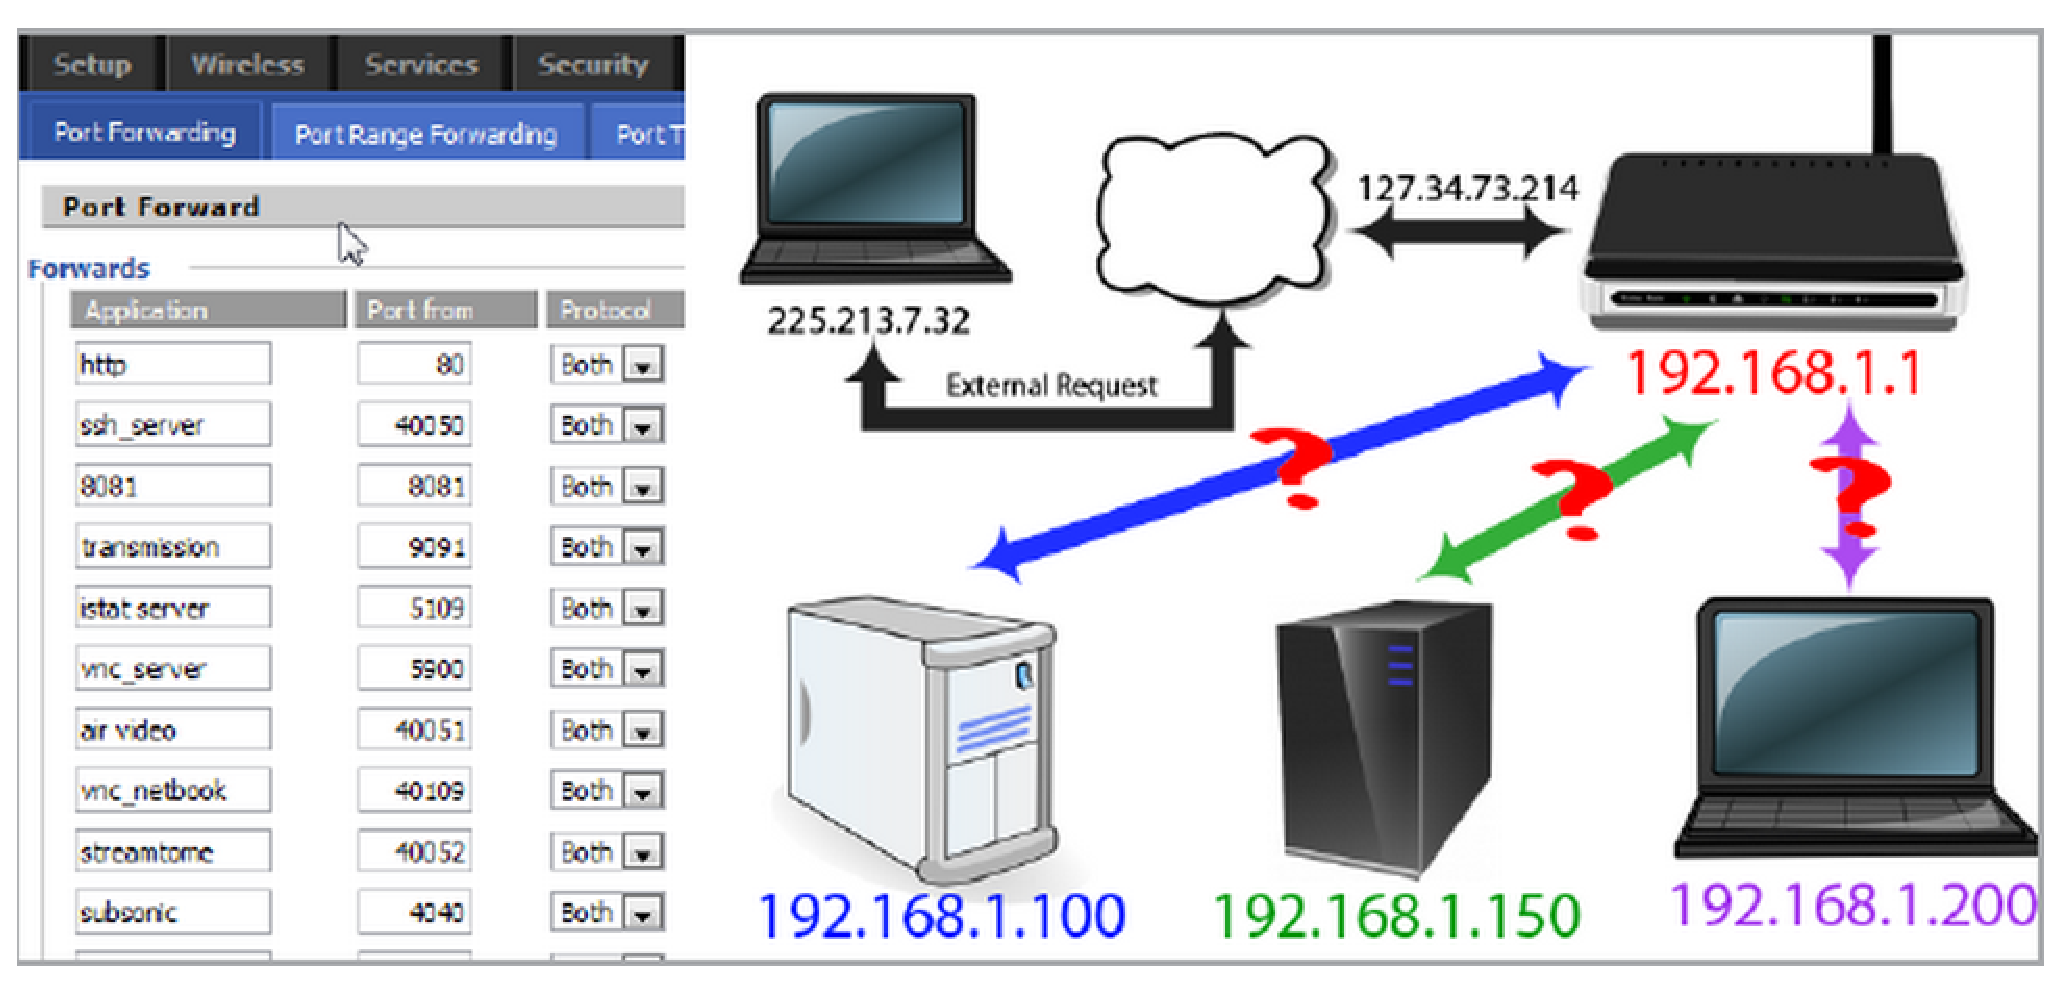
\includegraphics[height=5cm,
    angle=0]{./images/private_network.eps}}
  \caption{A private network}
  \label{fig:private_network}
\end{figure}

Make a diagram of your network
\begin{itemize}
  \item router: use circle with 4 arrows arranged in a cross
  \item switches: square or rectangle, with 4 staggered arrows, two in each
  direction
  \item hubs: same as switch, with a single double-headed arrow
  \item lines and squares to represent connection leading to computers
\end{itemize}
\url{http://www.wikihow.com/Set-up-a-Private-Network}

Each machine need to have an assigned IP and a fully qualified domain names
(FQDNs). We can manually assign a fixed static IP for a machine, or we can let
it to get the IP assigned to it by the DHCP server. DHCP is short for Dynamic Host
Configuration Protocol, a protocol for assigning dynamic IP addresses to devices
on a network.  Dynamic addressing simplifies network administration because the
software keeps track of IP addresses rather than requiring an administrator to
manage the task. 

A router or an ISP always has DHCP implemented. The DHCP server also provide its
clients with a DNS (Domain Name Server) service. A DNS can reside on the same or
different one with the DHCP server. DNS is an Internet service that translates
domain names into IP addresses. Because domain names are alphabetic, they're
easier to remember. For example, the domain name www.example.com might translate
to 198.105.232.4. 

\subsection{DHCP server }

You can choose to disable the DHCP server feature on your home router and set up
a Linux box as the DHCP server. Managing the DHCP daemon is easy to do, but the
procedure differs between Linux distributions.
\url{http://en.wikipedia.org/wiki/Comparison_of_DHCP_server_software}
\begin{itemize}
  \item \verb!dhcpd! daemon: managed by a daemon management system (e.g.
  \verb!SysV! or \verb!Systemd!)
\begin{verbatim}
// Redhat/CentOS/Fedora
rpm -ivh dhcp-x.xxx.elx.i386.rpm

// Ubuntu/Debian 8
apt-get install dhcp3-server 

// Ubuntu 11.04 + (part of Busybox package)
udhcpd 
\end{verbatim}
  
  To start DHCP server
\begin{verbatim}
// Redhat/CentOS/Fedora
service dhcpd start 
/etc/rc.d/init.d/dhcpd start

// Ubuntu/Debian
/etc/init.d/networking restart
\end{verbatim}
  
  To change the configuration
\begin{verbatim}
// Red Hat/CentOS/Fedora (DHCP v3.0.1)
vi /etc/dhcpd.conf
vi /etc/dhcp.conf  

// Ubuntu/Debian: 
vi /etc/default/dhcp3-server

\end{verbatim}


Example of the configuration file content
\begin{verbatim}
ddns-update-style interim;                                   # Required for dhcp 3.0+ / Red Hat 8.0+
ignore client-updates;

subnet 192.168.1.0 netmask 255.255.255.0 {
        range 192.168.1.128 192.168.1.254;                   # Range of IP addresses to be issued to DHCP clients
           option subnet-mask              255.255.255.0;    # Default subnet mask to be used by DHCP clients
           option broadcast-address        192.168.1.255;    # Default broadcastaddress to be used by DHCP clients
           option routers                  192.168.1.1;      # Default gateway to be used by DHCP clients
           option domain-name              "your-domain.org";
           option domain-name-servers      40.175.42.254, 40.175.42.253;           # Default DNS to be used by DHCP clients
           option netbios-name-servers     192.168.1.100;    # Specify a WINS server for MS/Windows clients.
#         DHCP requests are not forwarded. Applies when there is more than one ethernet device and forwarding is configured.
#       option ipforwarding off;
        default-lease-time 21600;                            # Amount of time in seconds that a client may keep the IP address
        max-lease-time 43200;
        option time-offset              -18000;              # Eastern Standard Time
#       option ntp-servers              192.168.1.1;         # Default NTP server to be used by DHCP clients
#       option netbios-name-servers     192.168.1.1;
# --- Selects point-to-point node (default is hybrid). Don't change this unless you understand Netbios very well
#       option netbios-node-type 2;
        # We want the nameserver "ns2" to appear at a fixed address.
        # Name server with this specified MAC address will recieve this IP.
        host ns2 {
                next-server ns2.your-domain.com;
                hardware ethernet 00:02:c3:d0:e5:83;
                fixed-address 40.175.42.254;
        }
        # Laser printer obtains IP address via DHCP. This assures that the
        # printer with this MAC address will get this IP address every time.
        host laser-printer-lex1 {
                hardware ethernet 08:00:2b:4c:a3:82;
                fixed-address 192.168.1.120;
        }
}
\end{verbatim}

  \item \verb!maas-dhcp! daemon: used by MAAS (Sect.\ref{MaaS_maas-dhcp})
\end{itemize}
You can define your server configuration parameters in the dhcpd.conf file which
may be located in the /etc the /etc/dhcpd or /etc/dhcp3 directories depending on
your version of Linux. 

\subsection{Port forwarding}
\label{sec:port_forwarding}

Port forwarding allows an machine form outside to use a service provided by  a
machine from inside a private the network.  The service can be SSH, HTTP.
\begin{itemize}
  \item SSH: port 22
  \item VNC: port 5900
  \item HTTP: port 80
\end{itemize}
\url{http://www.howtogeek.com/66214/how-to-forward-ports-on-your-router/}

The machine outside only know the single public IP of the router, and have no
idea about the local IP of the machine providing the service. So, we need to
tell the router to do port forwarding to the machine depending on which port of
the service is being requested. So, for a given service, if port 80 use machine
8, if port 8080 use machine B.

To configure port forwarding, we need to connect to the router. Depends on the
router brand, you can see different UI
\begin{itemize}
  \item Cisco/Linksys: Login, and
select \verb!Applications & Gaming!. and choose {\bf Single Port Forwarding}

  \item D-Link: Advanced, and choose Port Forwarding
  \item Netgear: Advanced/ Port Forwarding-Port Triggering
  \item DD-WRT: NAT/QoS and choose Port Forwarding
\end{itemize}
\begin{verbatim}
Application  External  Internal  Protocol        IP Address         Enabled
             Port      Port                     (local machine)
  HTTP        80        80       TCP            192.168.1.10           YES
  FTP
  FTP-data
  SSH
  SMTP
  NTP
  finger
  POP3
  Telnet
  SNMP
  NNTP
  CVS
\end{verbatim}
\url{http://www.howtogeek.com/66214/how-to-forward-ports-on-your-router/}


\section{PXE booting}
\label{sec:PXE_booting}

Network booting with PXE (Pre-boot eXecution Environment) allows you to boot up
a system and have it automatically get an IP address via DHCP and start booting
a kernel over the network.

In order to use PXE you need to setup a boot-server which will allow client systems to :
\begin{itemize}
  \item  Request an IP address (via DHCP)
  \item  Download a kernel (via TFTP)
\end{itemize}
\url{https://www.debian-administration.org/article/478/Setting_up_a_server_for_PXE_network_booting}

In BIOS

In UEFI (e.g. ASUS UEFI BIOS)
\begin{verbatim}
Advanced
   Network Stack
      IPv4 PXE support   (YES)
      IPv6 PXE support   (YES)
      
Advanced
   Onboard Devices Configuration
       Realtek PXE OPROM => Enabled
       
Boot 
   Boot Option Priorities 
      Boot Option #1 = DVDRAM             
      Boot Option #2 = UEFI: IP4
\end{verbatim}
\url{http://www.ccboot.com/uefi-bios.htm}

% \section{Network interfaces}
% \label{sec:network_interfaces}


\section{DHCP server}
\label{sec:DHCP}

A DHCP server provides a service to manage IP assigment to each machine in the
subnet. This can be provided by (1) the router/DHCP, (2) server/DHCP. In
general, you'd use a DHCP server if the extra load on the router loads it down.
Once a need was identified, the network administrator would plan a migration
from the router/DHCP to a server/DHCP.
\url{http://www.techexams.net/forums/network/91915-when-use-seperate-dhcp-server-vs-having-router-do-dhcp.html}
\begin{verbatim}
Router DHCP = small offices, homes and businesses
DHCP Server = enterprise, large businesses
\end{verbatim}

Softwares
\begin{itemize}
  \item \verb!isc-dhcp-server!
\begin{verbatim}
apt-get install isc-dhcp-server

$> vi /etc/dhcp/dhcpd.conf
## disable dynamic DNS
## prevent DHCP server from receiving DNS information
##    from clients
ddns-update-style none;

## Set a domain name for your LAN ##
option domain-name "nixcraft.net.in";
 
## Set DNS server IP address, you can set to your ISP's dns server too or use Google DNS server##
option domain-name-servers 192.168.1.2, 192.168.1.3;

### Set the length in seconds that will be assigned to a lease if the client requesting the lease does not ask for a specific  expiration time.   ##
### This is used for both DHCPv4 and DHCPv6 leases (it is also known as the "valid lifetime" in DHCPv6). ###
default-lease-time 86400;
 
## Set the maximum length in seconds that will be assigned to a lease ##
max-lease-time 604800;
 
 ## uncomment this
 ## i.e. DHCP server should send DHCPNAK messages to
 ##      misconfigured clients 
authoritative;

 ## Finally, update the subnet
subnet 192.168.1.0 netmask 255.255.255.0 {
        ## dhcp start  and end IP range ##
        range 192.168.1.100 192.168.1.200;
        option subnet-mask 255.255.255.0;     ## subnet 
        option broadcast-address 192.168.1.255; ## broadcast
        option routers 192.168.1.254; ## router IP
} 
  
\end{verbatim}

Restart the DHCP server
\begin{verbatim}
dhcpd -t /etc/dhcp/dhcpd.conf

service isc-dhcp-server start
service isc-dhcp-server stop
service isc-dhcp-server restart
service isc-dhcp-server status
 
\end{verbatim}
  \url{http://www.cyberciti.biz/faq/howto-ubuntu-debian-squeeze-dhcp-server-setup-tutorial/}
  
  \item \verb!maas-dhcp!
\end{itemize}


\section{Wake-on-Lan vs. IPMI vs. iLO}
\label{sec:power-remotely}

A workstation can be in one of the different 6 System Power States (S0-S5) -
Sect.\ref{sec:ACPI}. There are different methods to power on a standby machine
remotely. Different vendors have different methods for power management
\begin{itemize}
  \item  Intelligent Platform Management Interface (IPMI). 
  
  Currently only servers support this. Check your vendor documentation to see
  if IPMI is on your computer or not. \url{http://fish2.com/ipmi/ipmi_faq.html}
  
  \item Dell's iDRAC
  
  \item HP's Integrated Lights-Out (iLO) interface  
  
  \item IBM's RSA
  
  \item Wake-on-LAN (WOL): 
\end{itemize}


IPMI/iLO implies a "more reliable" mode of operation since it relies on
out-of-band management to activate the power-on event. Likewise, IPMI/iLO events
are more likely to span networks than WOL since WOL ultimately works at layer-2.
 If your vCenter is not directly connected to your WOL target network (i.e. ESX
hosts) you should opt for IPMI as the DPM management protocol for your DRS cluster.


\subsection{WOL}
\label{sec:Wake-on-Lan}

Wake-on-LAN is the protocol defined by AMD and HP for remotely
waking up a remote host. A MagicPacket is sent via either Ethernet
or UDP. There are two Unix programs, \verb!etherwake! works for Ethertype
0x0842 \footnote{\url{http://en.wikipedia.org/wiki/EtherType}} and
\verb!wakeonlan! for UDP.
\begin{itemize}
    \item \verb!etherwake!: can power on a remote host in soft-powered-down ACPI
    D3-warm state. \url{http://linux.die.net/man/8/ether-wake}
\begin{verbatim}
sudo etherwake -i <iface>  <MAC-address>

sudo etherwake -i p2p1   29:23:9A:1A:9B:94
\end{verbatim}
    
    \item \verb!wakeonlan!: UDP port 9
    
    \url{http://superuser.com/questions/295325/does-it-matter-what-udp-port-a-wol-signal-is-sent-to}
\end{itemize}  

  \url{http://wiki.wireshark.org/WakeOnLAN}
% There are two implementations to generate and transmit Wake-on-LAN  ``Magic
% Packet'', used for restarting machines that have been soft-powered-down (ACPI D3-warm state)
% \begin{itemize}
%   \item \verb!etherwake!: use Ethernet (Ethertype 0x0842), with package
%   is sent via the default \verb!eth0! interface. To specify a different
%   interface
%   
%   \url{http://linux.die.net/man/8/ether-wake}
%   
%   \item \verb!wakeonlan!: use UDP port 9, there is no way to change the
%   interface
% 
% \end{itemize}


Enabling WOL will most likely require a BIOS setting change in the power
management section. For PCI-E network adapters, the "Resume on PCI-E Wake" event
must be enabled.

To check if it is enabled on the current machine (make sure the output contain
'g')
\begin{verbatim}
$> sudo ethtool <NIC> | grep "Wake"

Supports Wake-on: g
Wake-on: g
\end{verbatim}
If the output contains 'd' it means we can enable it using the command (but it
doesn't survive reboots)
\begin{verbatim}
sudo ethtool -s <NIC> wol g
\end{verbatim}
\url{http://superuser.com/questions/524158/wakeonlan-and-etherwake-doesnt-work}


Configuring port forwarding on your router is a required change; WOL won't work
without it.

A physical WakeOnLAN (Magic Packet) will look like this:
\begin{verbatim}
6 bytes: Synchronization Stream
96 bytes: Target MAC address
0,4, or 6 bytes: Password (optional)
\end{verbatim}
The password field, if present, contains either 4 bytes or 6 bytes.
\url{http://wiki.wireshark.org/WakeOnLAN}


\subsection{IPMI}
\label{sec:IPMI}

IPMI is an acronym for a protocol: the Intelligent Platform Management
Interface. It helps manage what is sometimes known as Out-of-Band or Lights-Out
communication and is typically implemented by a chip or small set of chips on
the motherboard of modern servers.  

Pure IPMI is usually implemented as a network service that runs on UDP port 623
and often runs on a dedicated Ethernet port on the server.

\begin{enumerate}
  \item  IPMI v1.0 is no longer used.

  \item IPMI v1.5 added real networks (since 2001) with maximum password length
  is 16 characters (longer than that will be truncated). IMPI password management on
IMPI v1.5 is not recommended due to the unsecure format (clear text) that uses
to sent the password across the network. 

  \item IPMI v2.0 used maximum password length 20 characters (longer than that
  will be truncated). IPMI password management is only recommended on IPMI v2.0 lanplus
interface on the local station.
\url{http://h10025.www1.hp.com/ewfrf/wc/document?docname=c02604634&cc=us&dlc=en&lc=en}
  
\end{enumerate}

\subsection{iLO}
\label{sec:iLO}


\section{Routing table}
\label{sec:routing_table}

Your routing table is created automatically, based on the current TCP/IP
configuration of your Linux / UNIX computer. You can manually add / modify /
edit routing table using \verb!route! and \verb!ip! command. The types of
entries in a routing table:

\begin{verbatim}
$> route

$> route -n
\end{verbatim}
Consider the case you have two or more NIC cards, you need to tell the machines
which 
\begin{verbatim}
$> route -n
Kernel IP routing table
Destination     Gateway         Genmask         Flags Metric Ref    Use Iface
0.0.0.0         192.168.100.1   0.0.0.0         UG    0      0        0 p2p1
0.0.0.0         192.168.1.1     0.0.0.0         UG    0      0        0 p3p1
192.168.1.0     0.0.0.0         255.255.255.0   U     0      0        0 p3p1
192.168.100.0   0.0.0.0         255.255.255.0   U     0      0        0 p2p1

$> route 
Destination     Gateway         Genmask         Flags Metric Ref    Use Iface
192.168.1.0     *               255.255.255.0   U     1      0        0 eth0
192.168.122.0   *               255.255.255.0   U     0      0        0 virbr0
link-local      *               255.255.0.0     U     1000   0        0 eth0
default         192.168.1.1     0.0.0.0         UG    0      0        0 eth0
\end{verbatim}

\begin{itemize}
  \item The gateway is the IP address of the next router where a packet needs to be
sent. On a LAN link (such as Ethernet or token ring), the gateway must be
directly reachable by this router by using the interface indicated in the Interface
column. On a LAN link, both the gateway and interface determine how the traffic
is being forwarded by the router. For a demand-dial interface, the gateway
address is not configurable. On a point-to-point link, the interface determines
how the traffic is being forwarded by the router.

\begin{verbatim}
*                
0.0.0.0          (if -n is used)
      'unspecified' or 'there is none'
      It means the network is locally connected on that Interface
      and there is no next hop needed to get to it
      
\end{verbatim}
  \item Genmask: (Network mask) the combination of Genmask and Destination is
  used to determine the IP range
  
  \item Flags: 
\begin{verbatim}
U 
     router is Up
G
     the route is gateway
     (if not present, the route is a directly connected destination)
H     
     the destination is a complete host address
     (if not present, it is assumed the address can be a network address)
D     
     this route is created by a redirect
M     
     this route is modified by a redirect
A 
     (installed by addrconf)
C 
     (cache entry)
! 
     (reject route)     
\end{verbatim}
 \url{http://www.thegeekstuff.com/2012/05/route-flags/} 
  
  \item Metric: he relative cost of using the route to reach the destination. A
  typical metric is hops, or the number of routers to cross to reach the
  destination. If there are multiple routes with the same destination, the route
  with the lowest metric is the best route.  
  
  \item Protocol: the Protocol column lists RIP, OSPF, or anything other than
  Local, then the router is receiving routes. Open Shortest Path First (OSPF) is
  not available on Windows XP 64-bit Edition (Itanium) and the 64-bit versions
  of the Windows Server 2003 family.  
  
  \item Iface: Interface to which packets for this route will be sent.
\end{itemize}
\url{http://www.cyberciti.biz/faq/what-is-a-routing-table/}

Explanation:  any packet with a destination of 192.168.1.0 through 192.168.1.255
will be sent out \verb!eth0! without using a gateway
\begin{verbatim}
Destination     Gateway         Genmask         Flags Metric Ref    Use Iface
192.168.1.0     *               255.255.255.0   U     1      0        0 eth0
\end{verbatim}

Explanation: any packet with a link-local address
\begin{verbatim}
Destination     Gateway         Genmask         Flags Metric Ref    Use Iface
link-local      *               255.255.0.0     U     1000   0        0 eth0
\end{verbatim}
Link-local addresses are usually not guaranteed to be unique beyond a single
network segment. Routers therefore do not forward packets with link-local addresses.
\url{http://en.wikipedia.org/wiki/Link-local_address}

Explanation: any packet to a destination without another route will be sent out
eth0, using 192.168.1.1 as a gateway.
\begin{verbatim}
Destination     Gateway         Genmask         Flags Metric Ref    Use Iface
default         192.168.1.1     0.0.0.0         UG    0      0        0 eth0
\end{verbatim}
\url{http://stackoverflow.com/questions/8599424/understanding-routing-table-entry}

\section{Two gateways on one machine}

Suppose you have a machine with 2 NIC cards. Each of these cards has its own
default gateway, configured with 2 interfaces: \verb!eth0! and \verb!eth1!.

The two networks that should be used are 192.168.0.0/24 and 10.10.0.0/24,
whereby the first IP address in each respective network should be the gatewayv

\url{https://www.thomas-krenn.com/en/wiki/Two_Default_Gateways_on_One_System}


\section{Making your machine accessible from the Internet}
\label{sec:local_PC_accessible_via_Internet}


Your modem has a public IP. Your roter will assign private IP via DHCP or static
to one machine at home. 

Your public IP can change. Dynamic DNS is a free and useful way to keep track of
your Public IP address.  
Set yourself up with a free account and you'll have a fully qualified domain
name that won't change, even when your ISP changes your IP.
\url{www.dyndns.org}

If you have a Linksys or D-Link router, odds are that
it has Dynamic DNS (DDNS) functionality. Enable DDNS and enter your account
information into your router, and your router will keep your IP tied to your new
domain name. There are other Dynamic DNS services that also work.  

NOTE: If your router doesn't support Dynamic DNS, you can download a PC-based
client from Dynamic DNS to allow a PC on your LAN to keep your public IP
associated with your domain. However, your domain can't be updated if your IP
changes while your computer is turned off.

Static DHCP is a useful router configuration for a PC that you want to work with
remotely. I like this better than setting a static private IP. Static DHCP lets
your PC synch with the router and get the correct DNS information, saving the
hassle of configuring it on the PC.  

NOTE: Most routers allow you to specify a MAC address and assign it an IP
address. When properly configured, your PC will now always have the same IP, but get the
current and correct DNS IPs. Further, your router will have the MAC address of
the target PC stored in its config.  

\textcolor{red}{IMPORTANT:}Set up your router to allow for remote login. This is
a security concern, but it comes in handy while troubleshooting your home LAN
remotely. 
\begin{itemize}
  \item  The default setting on router and PC firewalls is to disable ping or echo
replies. Having this functionality enabled helps verify the reachability of your
LAN and PC. 
  
  If your PC firewall allows pings, it will come in handy when you're trying to
  see if your PC is on or off. 
\end{itemize}

\url{http://www.smallnetbuilder.com/lanwan/lanwan-howto/29941-how-to-wake-on-lan-wake-on-wan?showall=&start=2}

\url{http://wiki.networksecuritytoolkit.org/nstwiki/index.php/HowTo_Setup_A_Server_With_Multiple_Network_Interface_Adapters_Using:_"nstnetcfg''}

\section{Test bandwidth}
\label{sec:bandwidth-test}


On the listening-side (suppose its IP is 192.168.1.46):
\begin{verbatim}
$> nc -v -v -l -n -p 2222 >/dev/null
\end{verbatim}

On the sending-side
\begin{verbatim}
$>pv -t -r -a -b /dev/zero | nc -v -v -n 192.168.1.46 2222 /dev/null

Connection to 192.168.1.46 2222 port [tcp/*] succeeded!
 208MiB 0:02:15 [1.83MiB/s] [1.55MiB/s]
 233MiB 0:02:31 [1.83MiB/s] [1.54MiB/s]
 262MiB 0:02:51 [ 672kiB/s] [1.53MiB/s]
\end{verbatim}

\url{http://www.reddit.com/r/linux/comments/1maws6/checking_lan_transfer_speed_under_linux/}


\section{Network utilities}

\subsection{netcat, nc}
\label{sec:netcat}

Netcat has two forms:
\begin{itemize}
  \item netcat traditional

This is the "classic" netcat, written by *Hobbit*. It lacks many
features found in netcat-openbsd.

It has \verb!-e! option to execute program from remote shell, which is not
present in netcat-openbsd.
  
  \item netcat-openbsd:

 This package contains the OpenBSD rewrite of netcat, including support
 for IPv6, proxies, and Unix sockets.
 
 There is no -c or -e option in this netcat, but you still can execute a
 command after connection being established by redirecting file descriptors.
 \url{https://superuser.com/questions/691008/why-is-the-e-option-missing-from-netcat-openbsd}
 
 \item others???
 
 You have netcat versions from OpenBSD, FreeBSD, the GNU netcat, et cetera.
   
\end{itemize}
 
In a simple way, netcat is a telnet that you can use in scripts. Plus is can be
used as a simple listener if you want.

Netcat is like socat with only the STDIO, TCP, TCP-LISTEN, UDP, and UDP-LISTEN
address types with fewer options for those address types.

To listen on a given address, and a given port
\begin{verbatim}
nc -l -s <LISTENING_IP_ADDR> -p <LISTENING_PORT>
\end{verbatim}

To execute commands on remote machines
\begin{verbatim}
 Be cautious here because opening a port and let anyone connected execute
 arbitrary command on your site is DANGEROUS. If you really need to do this,
 here is an example:

 On 'server' side:

       $ rm -f /tmp/f; mkfifo /tmp/f
       $ cat /tmp/f | /bin/sh -i 2>&1 | nc -l 127.0.0.1 1234 > /tmp/f

 On 'client' side:

       $ nc host.example.com 1234
       $ (shell prompt from host.example.com)

 By doing this, you create a fifo at /tmp/f and make nc listen at port 1234
 of address 127.0.0.1 on 'server' side, when a 'client' establishes a
 connection successfully to that port, /bin/sh gets executed on 'server'
 side and the shell prompt is given to 'client' side.

 When connection is terminated, nc quits as well. Use -k if you want it keep
 listening, but if the command quits this option won't restart it or keep nc
 running. Also don't forget to remove the file descriptor once you don't
 need it anymore:

       $ rm -f /tmp/f
\end{verbatim}

\subsection{socat}
\label{sec:socat}



socat can do serial line stuff, netcat cannot. socat can do fairly advanced
functionality, like having multiple clients listen on a port, or reusing connections. 

SERVER SIDE:  telling it to listen for connections on port 3333. Each time it
receives a connection it will execute cat, redirecting and appending ('>>')
received input as output into the file /tmp/log.txt: 
\begin{verbatim}
socat tcp-l:3333,reuseaddr,fork system:'cat >> /tmp/log.txt',nofork
\end{verbatim}

SENDING SIDE:
\begin{verbatim}
socat - UDP4-DATAGRAM:20.21.22.23:2001

echo "SO MANY BEDS, WITH PHONES NEXT TO HEADS" | socat - UDP4-DATAGRAM:20.21.22.23:2001
\end{verbatim}

\url{https://discourse.criticalengineering.org/t/howto-crafting-arbitrary-network-packets-with-socat/51}